\section{Introduction}
Anybody who has been caught up in a sidewalk dance knows that human coordination without common knowledge about each other's intentions is prone to failure. Thus, cooperating humans have evolved techniques by which to create common knowledge in practice, such as eye contact, conventions, and broadcasted messages. When common knowledge cannot be obtained, humans routinely act upon their private knowledge, or upon their shared reasoning about other minds. While we know much about human limits to such higher-order belief reasoning, little is known about at which point, and under which circumstances, shared knowledge becomes effectively indistinguishable from common knowledge. We investigate this question with a novel recursive coordination game with imperfect information, and show that people consistently act as if they have common knowledge about a fact, even in situations where they share only the shallowest levels of their state of mind.  

Successful group coordination requires complementary choices among group members, which, in turn, requires communication of beliefs and intentions in such a way that they become common knowledge~\cite{fagin1995reasoning}. A fact is said to be \textit{common knowledge} if everyone knows it, and everyone knows everyone knows it, and everyone knows everyone knows everyone knows it, and so on, ad infinitum~\cite{lewis1969convention, clark1981definite, schelling1980strategy, aumann1976agreeing}. If the premise of  ``everyone knows'' is not infinitely nested, but only nested to finite depth, we instead have \emph{shared knowledge}. If there is no nested knowledge about knowledge at all and not everyone necessarily knows the fact, we have \emph{private knowledge}.

Let us illustrate the difference between these notions with an example. Two friends, Agnes and Bertram, are taking different trekking routes on the same mountain, and have agreed to meet at the top. 
%In the morning they agree that if the weather gets bad, they will go back down and sleep in the mountain hut at the base. Otherwise, they strongly prefer to stay overnight at the top. 
The equipment essential for an overnight stay at the top has been divided between their backpacks, so it's crucial for their safety that they meet there before it gets dark. 
%. It is therefore crucial that if one of them decides to go to the top, the other one does the same. 
On the way to the top, they both observe bad weather approaching, which makes it safer to go back to the base. However, they are both uncertain about whether the other person has seen the bad weather, so they cannot expect the other person to necessarily go to the base. The most dangerous situation is if one of them goes to the base and the other goes to the top, since then one of them is left at the top without the necessary equipment to stay there for the night. 

At this point they both know the fact that ``bad weather approaches'', but don't know whether the other knows. In this situation, we would say that Agnes and Bertram both have \emph{private knowledge} that bad weather is approaching, and since they both know it, it is also \emph{shared knowledge} between them. More generally, a fact is \emph{private knowledge} in a group of agents if some non-empty subset of the agents know the fact. For the special case where everybody in the group knows it, we say that there is \emph{shared knowledge to depth one} (or \emph{first-order shared knowledge}) of the fact~\cite{clark1981definite}. The exact border between what is considered private and shared knowledge vary between authors. Some consider the case where everybody knows a fact to still only be private knowledge, and that for it to be shared knowledge, at least one agent also needs to know that they all know. The notion of shared knowledge we use in this paper, where shared knowledge only requires that everybody knows, is the one originally used by~\cite{clark1981definite}, and also the one often seen in (epistemic) logic~\cite{herzig2015share}. Formal definitions of private, shared and common knowledge as well as a more detailed discussion of our choice of conventions can be found in Appendix \ref{A:definitions}. 
%\footnote{\supplementary_name is accessible at \url{http://www2.compute.dtu.dk/\~tobo/cd_sm.pdf}.}

Since Agnes doesn't know whether Bertram knows about the bad weather, she would like to warn him and suggest to meet back at the base. So she sends a text message: ``Bad weather approaching. Let's meet at base.'' However, due to the unstable mobile network signals, she is not certain that the message will go through. Therefore she asks Bertram to confirm that he received the  message. A few minutes later, she receives his confirmation. At this point it has become \emph{shared knowledge to depth two} (or \emph{second-order shared knowledge}) that bad weather is approaching: He knows that she knows, since he received her message, and she knows that he knows, because she received his confirmation. To have \emph{shared knowledge to depth three} (\emph{third-order shared knowledge}), it would additionally be required that A) she knows that he knows that she knows, and B) that he knows that she knows that he knows. In fact, A already holds, since she received (and read) his confirmation. However, B doesn't hold, since he will be uncertain about whether his confirmation was successfully received. Thus we have asymmetry in the level of knowledge of the two agents. If he also asks her to confirm his message, and he receives such a confirmation, then of course he will get to know that she knows that he knows. Then there will be shared knowledge to depth three. However, there will still be a (higher-order) knowledge asymmetry, since Agnes can't be certain that the last message was received.

How many messages back and forth does it take for Agnes and Bertram to coordinate going back to the base? At first it might seem that it is sufficient for both of them to know that at least one of them plans to go to the base. However, that is not so. After the first message has been received, both know that Agnes plans to go to the base, but she is still uncertain whether he knows. And if he doesn't, she might risk leaving him alone at the top. So shared knowledge to depth one is clearly not sufficient. Even shared knowledge to depth two is not sufficient. After he has confirmed receiving her original message, from his perspective it is still entirely possible that she doesn't know that he knows, and hence, she might decide to go to the top to not leave him alone up there. And in this case, he also has to go to the top in order not to leave \emph{her} alone up there. This argument can be generalised to prove that even $n$th-order shared knowledge for any arbitrary large $n$ is insufficient for safe coordination.\footnote{To derive a contradiction, suppose $n$th-order shared knowledge for some $n$ is sufficient to make it safe to go to the base, in the sense of guaranteeing that the other person will also go there. This implies that the successful delivery of the $n$th message is sufficient to guarantee meeting at the base. There must then exist a smallest number $n_0$ such that the successful delivery of the $n_0$th message is sufficient to guarantee meeting at the base. Since $n_0$ is the smallest such number, the successful delivery of the $(n_0-1)$st message is not sufficient to guarantee meeting at the base. Now note that at the moment when the $n_0$th message has been successfully delivered, the sender of this message is still uncertain about whether it was actually received, and hence the sender is only certain that the first $n_0-1$ messages has been successfully delivered.  In other words, the sender of the $n_0$th message considers it possible---even after the successful delivery of the message---that only the first $n_0-1$ messages were successfully delivered, in which case it is \emph{not} safe to go to the base. Hence that person will after having sent the $n_0$th message stil consider it unsafe to go to the base, and will choose to go to the top. This is a contradiction, completing the proof. This proof is stated in rather informal terms, but can be turned into a formal, mathematical proof~\cite{fagin1995reasoning}. The example here is in fact modelled after the coordinated attack problem studied extensively in that book, where it is also used to illustrate that common knowledge is a necessary condition for coordination. We are making a similar point here about the necessity of common knowledge for coordination, just using another example.}  The consequence is that no finite number of messages successfully delivered will guarantee that Agnes and Bertram manage to meet at the base. In order to guarantee meeting at the base, they would need to have shared $n$th-order knowledge for \emph{all} $n$. Shared $n$th-order knowledge of some fact for all $n$ is called  \emph{common knowledge} of the fact (see again  %the 
Appendix \ref{A:definitions} for a more formal definition). The essence of the argument is that any  
%\add{This is highly intuitive, but the fact remains that any 
plan for Agnes and Bertram to coordinate without common knowledge would leave one stranded at the top in the case of a faulty signal at a critical point in their communication.
%}

In practice, shouldn't it be possible to coordinate meeting at the base after one or two messages being sent back and forth? It is likely that this is what Agnes and Bertram would attempt, at least. The question is whether they are fully aware of the risk of miscoordination in this case? After Agnes has sent the message and Bertram has successfully confirmed receiving it, are they aware that the content of the message is still not common knowledge, and that they still risk miscoordination? Or do they now believe it completely safe to go to the base? The questions here are whether A) they can distinguish between the case of $n$th-order shared knowledge and common knowledge, and whether B) they would act differently in the case of common knowledge than in the case of $n$th-order shared knowledge for some suitable large $n$. 
% as if they have common knowledge despite only having $n$th-order shared knowledge.    


% Isn't it a purely mathematical problem with no practical implications for humans trying to coordinate their actions? One of the main goals of this paper is to argue that the answer to both questions is no. \tsn{Skal vi ændre formuleringen så vi ikke direkte påstår det har praktiske implikationer ift mennesker, men mere beskriver at det har konsekvenser i det omfang sådanne problematiske epistemiske strukturer findes, selvom (eller specielt derfor), at vi ikke kan indse at de er problematiske (som vores forsøg viser, og som er tydeligt når selv i mountrain-trekking eksemplet er mange kritiske)} 
%In order to make that argument, 
We have designed a coordination game that has a similar underlying mathematical structure as this trekking example, but cast in a simpler setting, where the higher-order uncertainty is established already when the game is initialised and not, as above, through a series of message passings. In this game, our experiments show that human players indeed try to coordinate on the preferred outcome even when only having low orders of shared knowledge (corresponding to trying to meet at the base after only a  few message passings in the trekking example). However, this often results in severe cases of miscoordination with high penalty, corresponding to the situation in the trekking example where one of the trekkers would leave the other at the top without the necessary equipment. Our game suggests that the answer to B above is sometimes a ``no'': Most players definitely act as if they have common knowledge, even though they don't, i.e., for sufficiently high levels of shared knowledge, they act as in the common knowledge situation. For sufficiently high levels of shared knowledge, they play strategies that would have given them the highest payoff if they had had common knowledge, but since they don't, they end up with payoffs that are significantly lower than what they could have received if they had explicitly distinguished the common knowledge situation from the $n$th-order shared knowledge situation. One might however still speculate that this is a 
%Despite this not leading to the game-theoretically optimal strategy, we might speculate that it is nevertheless a 
conscious choice of strategy, and that the players are nevertheless aware that they don't have common knowledge. However, through follow-up questions and interviews, it seems that the answer to A is also ``no'': Players claim they have common knowledge and that coordination is guaranteed, even when they only have low-order shared knowledge.     

Humans generally find the concept of common knowledge hard to grasp, and even harder to grasp the practical relevance of, due to the unbounded nesting of knowledge. We originally developed our game to illustrate that the difference between $n$th-order shared knowledge and common knowledge can have actual strategic implications, hence helping to understand the notion of common knowledge better (and why $n$th-order shared knowledge for sufficiently high values of $n$ is not sufficient). The game we developed makes it clear that human intuitions about common knowledge can be misleading and may have costly consequences.

\section{The curse of shared knowledge}
Reasoning about the knowledge of others, their reasoning about you, and your reasoning about their reasoning, and so on, is famous in cognitive science for its presumed computational intractability~\cite{van2018parameterized,bolander2023parameterized}. Because of this, coordinating species typically use heuristic shortcuts in order to reduce complex shared knowledge states, such as joint perceptual cues and broadcasted signals~\cite{milgrom1981axiomatic, clark1996using, bradbury1998principles}. Humans may obtain common knowledge via mutually accessible first-order sensory experiences~\cite{tomasello1995joint, lorini2005establishing, bolander2015announcements, gintis2010rationality}, eye contact~\cite{friedell1969structure}, public rituals and conventions~\cite{lewis1969convention}, or salient focal points~\cite{schelling1957bargaining}. What most prominently is believed to distinguish human coordination from other animals, however, is the enormous flexibility by which humans can imagine and articulate the mental states of their peers~\cite{tooby2010groups, harari2014sapiens}. The abilities to blush, to tell jokes, and to write novels testify that humans readily attribute \textit{higher-order} beliefs, intentions, and reasoning capabilities to other people, such as thinking explicitly about the mental states of others who think about the thoughts and beliefs of others and so on---while at the same time appreciating that those thoughts and beliefs can differ from each other and from reality. Such higher-order cognition has seen substantial scientific attention, and has brought about various technical terms such as ``Theory of Mind'' (ToM)~\cite{premack1978does}, ``mentalizing''~\cite{frith2003development}, ``mind reading''~\cite{vogeley2001mind, apperly2010mindreaders}, %``mental models''~\cite{johnson1983mental},
``mind perception''~\cite{gray2011distortions}, ``perspective taking'', and ``social intelligence''~\cite{baron1999social}, which often are used interchangeably for studying the cognitive mechanisms of shared knowledge, but sometimes focus on slightly different ideas and associated meanings~\cite{schaafsma2015deconstructing}, depending on the field of investigation.

Looking at the ToM-literature, conclusions about human belief reasoning abilities are rather heterogeneous~\cite{apperly2009humans, saxe2013theory}: Human reasoning about the reasoning processes of other humans is limited~\cite{premack1978does, gopnik1988children, stahl1995players, nagel1995unraveling, hedden2002you, keysar2003limits, pinker2003language}, contextual, and possibly domain specific~\cite{leslie1992domain, saxe2009theory, heyes2014submentalizing}. Three-year-old children tend to fail in the well-known first-order false belief tasks by falsely assuming that their private information is shared by others, while second-order false belief tasks are mastered around ages 5-7~\cite{perner1985john, sullivan1994preschoolers}. Adults may reliably master up to four orders~\cite{kinderman1998theory}, but still have difficulties ignoring the private information they possess when assessing the beliefs of others, resulting in a \textit{curse of knowledge} bias which can compromise their ability to make predictions about other people’s beliefs and actions~\cite{camerer1989curse, birch2007curse}. When the nested mental states represent a succession of different people, such as ``Alice thinks that Bob thinks that Carol is contemplating the idea that David is thinking about Evelyn'', we have less problems following along\footnote{Especially when those successions of mental states are qualified by psychological attribute words such as `Alice thinks that Bob is mistakenly worrying that Carol is offended by misunderstanding something Dave had said to Evelyn'.~\cite{academian2019unrolling}.
} than when the nested mental states are successions of the same people over and over again, and thus are truly recursive, such as ``I think that you think that I contemplate the idea that you are thinking about me''. We get confused more easily by the latter formulation, since we need to keep track of several representations of ourselves and of the other, each representation differing in its perspective and in the number of mental states it presupposes~\cite{de2019common}. When humans compete or try to detect cheaters, higher-order belief reasoning seems to perform better than lower-order belief reasoning~\cite{goodie2012levels}. In negotiations and other mixed motive situations, where innuendo, threats, bribes and other kinds of indirect propositions are common, humans are very good at the \textit{strategic} use of higher-order belief reasoning, for instance as a means to \emph{prevent} common knowledge in certain groups of agents, or as a means to form specific knowledge alliances~\cite{pinker2007stuff, pinker2008logic, de2017negotiating}. ToM proficiency may also be facilitated by providing games with stepwise increase in ToM~\cite{verbrugge2018stepwise}.

In pure coordination problems, such as pedestrians choosing sides, or people agreeing on new words or on new technical standards, common knowledge is the normatively preferred informational state for all members of the group, because it allows to coordinate on an optimal common equilibrium. If there are no or limited means by which to communicate, however, people face an equilibrium-selection problem for which neither game theory nor the ToM literature has any clear solution. Although some experimental evidence~\cite{curry2012putting} suggests that higher-order ToM reasoning may improve coordination efforts, other work seems to suggest that coordination favours lower orders of ToM sophistication~\cite{ devaine2014theory, de2015higher}. The challenge of tacit coordination is particularly relevant for artificial intelligence research and for social cognitive robotics, where the implementation of ToM-like processes into artificial social agents is believed to be an important step towards reliable human-robot interaction~\cite{erb2016artificial, bolander2018seeing, bard2020hanabi, dissing2020implementing}.

Recently, researchers have investigated whether humans have adapted specifically to recognizing common knowledge as a separate cognitive category, distinct from both private and shared knowledge~\cite{de2019common}. Controlled pure coordination experiments in social settings on market collaboration~\cite{thomas2014psychology}, the bystander effect~\cite{thomas2016recursive}, indirect speech~\cite{lee2010rationales}, self-conscious emotions~\cite{thomas2018common}, and charity~\cite{de2019maimonides}, consistently find that people indeed make strategically different choices under common knowledge conditions (presented in the form of public announcements), compared to situations in which there is only private knowledge (in the form of private messages) or shared knowledge (private messages that elaborate on the depth of knowledge of other participants). Apart from seeing a clear benefit of common knowledge, some of these studies also showed that people have a hard time discriminating between various orders of shared knowledge, and that coordination efforts do not correlate with payoff conditions~\cite{thomas2014psychology}, which is in contrast to the assumptions of standard rational choice theory in which payoffs are expected to be maximized~\cite{becker1976economic}.

Most of these studies are designed one way or the other to determine how far people typically unpack shared knowledge and whether they can recognize common knowledge when presented with it. They show that humans are indeed able to discriminate common knowledge from shared knowledge, and adapt their actions accordingly, at least in cases where it is simple to discriminate between the two states of knowledge. The purpose of our paper is somewhat different. The purpose is not to determine whether players can for instance distinguish $n$th order and $(n+1)$th order shared knowledge, but whether they can in general distinguish shared knowledge (of some order) from common knowledge. In the above-mentioned experiments, common knowledge was achieved via public announcements, and shared knowledge via private announcements in which the depth of knowledge was explicated. In other words, these were experiments in which the distinction between shared and common knowledge was made clear and explicit. The question then remains how good humans are at recognizing the difference between shared and common knowledge when the difference is not made explicit, but has to be deduced? The fact that humans are able to adapt their actions to whether they are in a shared or common knowledge situation might have significantly less practical relevance if humans in general have a hard time to distinguish these in the wild. The results of this paper suggest that humans are indeed not very good at recognizing the difference, in particular that they are prone to mistake $n$th-order shared knowledge for common knowledge---even for relatively low values of $n$. Or, at least, they behave as if they had common knowledge even when they only have $n$th-order shared knowledge for very moderate values of $n$. % \tsn{Skal det ændres, så vi siger at de enten ikke kan kende forskel, eller ikke ved om deres medspiller kan?}
This issue has not been thoroughly investigated in previous research, in part because many existing experimental designs stop after describing 2-3 orders of belief reasoning to the participants, as higher orders require quite convoluted sentences that tend to become incomprehensible and increase experimental error. Or, as in the mountain trekking example, they require reasoning about the consequences of a high number of (message passing) actions that each change the mental state of the involved agents.

The latter has been explored theoretically in the  `electronic mail game' by Rubinstein~\cite{rubinstein1989electronic}, a game version of the mountain trekking example and of the structurally equivalent `coordinated attack problem'~\cite{fagin1995reasoning}. The Rubinstein paper shows that `almost common knowledge' in the sense of $n$th-order shared knowledge for some large $n$, leads to a very different expected player behaviour than `absolute common knowledge'. Essentially his conclusion, translated into the context of the mountain trekking example, is that common knowledge is expected to make the two mountain hikers both go to the base, whereas if there is only $n$th-order shared knowledge for some $n$, they are expected to both meet at the top, independent of $n$ and despite the bad weather condition (resulting in non-maximal payoffs). Rubinstein does a pure game-theoretic analysis of optimal strategic behaviour in the game with no experiments, and only speculates what people playing the game might do. This paper aims at elucidating what actual human intuitions command in situations like this. Which depth of shared knowledge (if any) would be enough to attempt risky coordination that would lead to maximal payoff if successful? 

The electronic mail game and the mountain trekking example are complicated in terms of the dynamics of iterated message passing. In this paper, we devise a novel game in which the higher orders of shared knowledge are not achieved dynamically via actions, but are already present at the beginning of the game, using uncertainty about arrival times. This, we believe, makes the game easier to understand. Letting humans play our game, we have been able to address the previous questions in more detail. Our results indicate that the lack of common knowledge does not defer people from being confident in their ability to coordinate, except at the very lowest depths of shared knowledge. So people behave as if having common knowledge, despite only having a low level of shared knowledge, and despite the significant payoff penalties incurred. % \tsn{Skal vi bløde det her op, ift at usikkerheden om medspillere måske også har en rolle?}
%that the lack of common knowledge does not defer people from behaving as if they had common knowledge, resulting in significant payoff penalties.
%show that people indeed have a hard time accepting the fact that common knowledge is not reducible to shared knowledge of finite depth. \tobo{Again, the question is if this conclusion is too strong? Only our "do you have common knowledge" question actually indicates this. Also, of course, when I've talked to people, they claimed to have common knowledge, but we don't have data to back it up. We can say that our results "indicate" or something, but "show" is maybe too much. But what is true, of course, is that people behave *as if* they had common knowledge, and they even claim to be as certain about their actions *as if* they had common knowledge.} \tsn{Good point. We could angle it a bit towards behaviorism, and say that our results show that the lack of common knowledge does not seem to defer people from attempting to coordinate, except at 1-2 depths of shared knowledge. And then maybe that this indicates that people cannot distinguish between correctly between common knowledge and shared knowledge of certain depth. Consider "Our results show that people indeed behave as if they have common knowledge at sufficiently high levels of shared knowledge, resulting in significant payoff penalties.} \re{Enig. Jeg kan godt lide TSNs ændringsforslag: "Our results indicate that the lack of common knowledge does not defer people from attempting to coordinate, except at 1-2 depths of shared knowledge", og så fjerne den næste sætning der starter med "on the contrary..."} On the contrary, participants try to coordinate even at very low depths of shared knowledge and in spite of huge payoff risks. 
Our conjecture is that the sole presence of shared knowledge is enough to make participants try to coordinate, and that moderate depths of shared knowledge become effectively indistinguishable from common knowledge. 
%due to the recursive nature of the game. 
Our follow-up interviews seem to confirm this conjecture. 
We call this effect ``the curse of shared knowledge'' because even small depths of shared knowledge raises the participant's expectation of being able to coordinate in spite of repeated payoff penalties for having miscoordinated before.

\section{Experimental Design: Materials and Methods}\label{sect:experimental_design} 
\modified{We conducted three classroom experiments\footnote{\modified{The full version of this paper~\cite{bolander2025curse} also reports an online experiment with 680 participants on Amazon Mechanical Turk (MTurk). It is left out here, since on MTurk the players in principle cannot be guaranteed that their co-players have seen the same rules, or that they are even human, so the rules might not be common knowledge.}}}, with respectively 80 students (DTU1: $n=2160$) from the Technical University of Denmark (DTU) taking a course on Artificial Intelligence and Multi-Agent Systems, 42 students (DTU2: $n=1012$) taking an introductory course in Artificial Intelligence, and 12 students (DIS: $n=180$) taking a course on Artificial Intelligence at DIS---Study Abroad in Scandinavia (DIS). \modified{In the two DTU classroom experiments, the students got an initial endowment of \$30 and played 30 rounds (see below).} Also, in the DTU classroom experiments, all students were told that they would not receive any monetary rewards for playing the game, but they should still try to do their best. \modified{The rules were shown on a common screen and read aloud to the students, as in the DIS experiment (see below), so the rules of the game were common knowledge in all three experiments.} The students also had to answer a few additional post-game questions (see  Appendix \ref{app:dtu-experiments} for a full list of those questions). The DIS classroom experiment also differed in the formulation of the game itself, and the way it was presented to the students, see details further below. 

The experiment is designed as a two-player coordination game with imperfect information. The game is inspired by the structure of the consecutive number riddle, also called the Conway paradox, see e.g.\ \cite{van1980conway,van2015one}. Our game is framed as an everyday situation, where two colleagues arrive at their workplace in the morning, and have to decide whether to meet in the canteen for a morning coffee or go straight to their offices and start working immediately. We call the game the `Canteen Dilemma'. The purpose of framing it in an everyday situation is to attempt to make some of the recursive reasoning easier to comprehend~\cite{meijering2010facilitative, wason1971natural}. The introductory story of the game goes as follows: 
\begin{quote}
\indent
``Every morning you arrive at work between $8{:}10$ am and $9{:}10$ am. You and your colleague will arrive by bus 10 minutes apart. Example: You arrive at $\textbf{8:40 am}$. Your colleague may arrive at $\textbf{8:30  am}$, or $\textbf{8:50 am}$. Both of you like to meet in the canteen for a cup of coffee. If you arrive before 9:00 am, you have time to go to the canteen, but you should only go if your colleague goes to the canteen as well. If you or your colleague arrive at 9:00 am or after, you should go straight to your offices.''
\end{quote}




The game has three possible outcomes in each round: 1) both choose the canteen which we refer to as \emph{coordination into the canteen}; 2) both choose their respective offices which we refer to as \emph{coordination into the offices}; 3) one chooses the canteen and the other chooses the office which we refer to as \emph{miscoordination}. At the beginning of each round, participants are told only their own arrival time, and based on this they will have to decide whether to go to the canteen or to the office. After choosing one of those, participants are asked to estimate their certainty that their colleague will make the same choice (on a five-point Likert scale). 

\modified{Bonuses are calculated as penalties subtracted from the initial endowment of \$30 in each round.} Payoffs are tiered in such a way that a small penalty is deducted for successful coordination into the canteen (achieving the highest payoff), which is doubled for coordination into the offices (achieving the second-highest payoff), while the penalty for miscoordination or forbidden choices, i.e., going to the canteen at 9 am or after, is much larger (up to 921 times larger, meaning a significantly lower payoff than the previous two). This means that if a pair of players miscoordinate often, they risk loosing all their endowment, in which case their game terminates prematurely. Penalties are calculated by a logarithmic scoring rule, which depends on the decision and the certainty estimate by each player. Using penalties instead of bonuses may at first seem an unintuitive way to reward participants, but logarithmic scoring rules have been shown to work well due to their ability to ensure that loss minimization remains central, and that the players' actions represent their actual beliefs~\cite{good1992rational, seidenfeld1985calibration, palfrey2009eliciting, mccutcheon2019favor}. %In addition, we note that logarithmic scoring is a ``strictly propper scoring rule'' and generally does not create a cognitive overload \tobo{shouldn't there be a citation here?}. 
As noted in Appendix~\ref{appendix:payoffs}, we find a good match between certainty estimates and choices at arrival times different from those that are prone to miscoordination. This corroborates that players tried to minimize their losses and that they made their choices and certainty estimates as honestly as possible. 

We included payoff examples of both successful and failed coordinations in the instructions shown to the participants before the game started, as well as during the game in each round. Screenshots and full descriptions of the experimental setup can be found in Appendix \ref{app:mturk-walkthrough} and details of the payoff structure are provided in Appendix~\ref{appendix:payoffs}. % Payoffs and Penalties.

The DIS classroom version of the game experiments were different, since we wanted to test the robustness of our findings against variations in the specific formulations of the game and its setup. \modified{Additionally, we wanted to address a specific potential criticism of the original game setup. One might speculate} that the formulation of the game might create a certain behavioural bias, for instance a bias towards going to the canteen due to a personal preference for coffee over office. In the DIS classroom experiments, the following rules were presented publicly by being shown on the classroom projector and read aloud (see Appendix~\ref{app:dis-rules-full} for the full version): 
\begin{quote}
\indent
The 2 players have to try to coordinate their actions, and if they are successful, they will both achieve the same positive reward [...]. The positive reward can either be \$1 or \$2. If you’re miscoordinated, you lose all the money you earned so far in the game. [...] 
  
In each round, each player is dealt a face down card. On the face of the card there is a number in the interval 2-10 [...]. The numbers on the two dealt cards are always exactly 1 apart, so if for instance one of the players gets a 3, then the other will either be getting a 2 or a 4. [...] 

When the cards are dealt, each player looks at the number on their own card without showing it to the other. The two players are not allowed to communicate or exchange any kind of information during the game. After each player has inspected their own card, they should hide either a white or a black marble stone in their hand and put the hand on the table. [...] 

Both players then receive rewards depending on the colors of their stones and the numbers on their cards. The white marble stone is worth \$2, and the black marble stone is worth \$1, but you only get to keep your stones (money) if you choose the same stone as the opponent, and additionally, if you both choose the white stones, you only get to keep them if both card numbers are strictly below 9. In more details:  
\begin{enumerate}
  \item[a)] If one player chose a white stone and the other a black stone, then they both lose all the stones (money) they have received in the game so far.    
  \item[b)] If both players chose a black stone, they both receive \$1 (i.e., a black stone). 
  \item[c)] If both players chose a white stone, then they both receive \$2 (i.e., a white stone), but only if both numbers are strictly below 9, meaning they are both in the interval 2-8. If not, the players lose all the money (stones) they have received in the game so far.
\end{enumerate}
\end{quote}
This new version of the game is structurally equivalent to the original, but now formulated in a completely abstract way. This potentially makes it harder to grasp the rules, but avoids the potential problem of players making choices affected by everyday personal preferences. The reward structure is different in this version of the game. Instead of logarithmic scoring, we chose a simpler scoring with an even higher penalty (lose everything) for miscoordination (different stones) and ``forbidden'' choices (choosing white when having 9 or 10). This might help making it more clear to the players that choosing white is never worth the risk of miscoordination. % (more in this in the section on Game Strategies below).

The overall point of both versions of the game is that the only `safe' strategy is to always coordinate on the choice that gives the lower payoff (going to the offices or choosing black stones). Even if it seems safe to try to coordinate for the higher payoff when arriving sufficiently ahead of 9:00 am or getting a card with a number sufficiently below 9, it is never common knowledge that both arrived before 9:00 am or both have a card below 9, which makes it unsafe to attempt coordinating for the higher payoff. 


%ose everything), which should help making the players aware that avoiding miscoordination is the crucial aspect of the game. 
%\add{We also conducted a third alternate version of our experiment with 12 students (DIS: $n=180$). This was based on the Consecutive Numbers Riddle \cite{van2015one}, which our game was originally based on. Players got points (a figurative \$2 for coordination with white stones, \$1 for coordination with black stones, and losing all their earnings if miscoordinating. The players with highest got some nominal prize. This was to evaluate whether the framing of the game influenced player behavior (such as a natural preference for coffee over offices). We interviewed participants following the game, which we will discuss later in \nameref{discussion}.}. \tsn{TODO: Skal det beskrives nærmere? Transcript og lydfiler skal uploades ved submission, eller ind et sted?}


\section{Game Strategies}
What are the relevant strategies for this game? First note that going to the canteen at $9{:}00$ or after results in the worst possible payoff. So both players should always go to the office if they arrive at $9{:}00$ or after. How about if both arrive strictly before $9{:}00$? If both choose canteen, they getter a better payoff than if both choose office. Now consider a case where you are one of the players, and you arrive at $8{:}50$. Then your colleague will be arriving at either $9{:}00$ or $8{:}40$. If your colleague arrives at $9{:}00$, she has to choose office according to the previous argument, and then you would have to choose office as well to avoid the large penalty of miscoordination. However, if your colleague arrives at $8{:}40$, you may both choose the canteen, and this will lead to the highest payoff. In other words, depending on the arrival time of your colleague, a piece of information that you don't have access to, the best choice is either office or canteen. So which one to choose?

Since the penalty of miscoordination is very high, it would seem best to choose office. What if you then instead  arrive at $8{:}40$? In this case, your colleague either arrives at $8{:}30$ or $8{:}50$. In both cases, you have time to meet for a cup of coffee in the canteen, and doing so will give you the highest payoff. At first, it might seem like an easy choice. However, we just concluded that the best strategy at $8{:}50$ would be to go to the office. So, if you arrive at $8{:}40$ and contemplate that your colleague might arrive at $8{:}50$---and if you believe your colleague would reason as yourself and go to the office at $8{:}50$---you also ought to go to the office at $8{:}40$. This argument can of course be iterated, because if the optimal choice at $8{:}40$ is to go to the office, then the optimal choice at $8{:}30$ must also be to go to the office. In other words, the optimal strategy seems to be to always go to the office, independent of arrival time! And, indeed, so it is. If both players go to the office in all rounds and declare the highest possible certainty in their decisions, \modified{they will both leave the experiment with \$29.40 (see again Appendix~\ref{appendix:payoffs} for details of the payoff structure).} This is the highest possible payoff that can be guaranteed by any strategy in the game, and \modified{very close to the \$30 that the players start out with.} As we will see later, the payoffs that people actually get when playing the game are \emph{significantly} lower than this.

The \emph{all-office} strategy described above, where you always decide to go to the office independent of arrival time, is a safe strategy if both players follow it. By safe is meant that there is never any risk of miscoordination, and hence no risk of getting the highest penalty (the penalty for miscoordination is up to \$9.21 in a single round, see Appendix~\ref{appendix:payoffs}). It is actually the \emph{only} safe strategy. The reason is that if at least one of the players, say $a$, has the strategy of going to the canteen at some time $t$ before $9{:}00$, then since they both have to go to the office at $9{:}00$ or later, there must exist at least one pair of arrival times for which the two players are miscoordinated.\footnote{
\label{footnote:no-cutoff}  
We now prove this claim. Suppose $a$ has the strategy of going to the canteen at some time $t$ before $9{:}00$, and that both $a$ and $b$ will go to the office if they arrive at $9{:}00$ or later. To derive a contradiction, suppose $a$ and $b$ are always coordinated, i.e., always make the same choice for any pair of arrival times. Since $a$ chooses to go to the canteen at time $t$, player $b$ also has to go to the canteen at time $t+0{:}10$, since otherwise whey would be miscoordinated when $a$ arrives at $t$ and $b$ at $t+0{:}10$. But if $b$ goes to the canteen at time $t+0{:}10$, $a$ also has to go to the canteen at time $t+0{:}20$, since otherwise they would be miscoordinated when $b$ arrives at $t+0{:}10$ and $a$ at $t+0{:}20$. This can be generalized to conclude  that $a$ would have to go to the canteen at any time $t+0{:}20x$ for $x \geq 0$ and $b$ would have to go to the canteen at any time $t+0{:}10+0{:}20y$ for $y \geq 0$. Clearly this implies going to the canteen after $9{:}00$, which is a contradiction.}

The fact that the all-office strategy is the only safe one is counter-intuitive to most people before being presented with the proof, and for some people even after. The issue is that, intuitively, it would seem to be safe to go to the canteen at, say, $8{:}30$. Why would a person/player, say Agnes, ever go to the office that early? She knows that her co-player/colleague, say Betram, will then be arriving at latest at $8{:}40$, which still leaves plenty of time to get a cup of coffee together before $9{:}00$. The issue is of course that if Agnes takes the perspective of Bertram, then assuming he arrives at $8{:}40$, he will consider it possible that she arrives at $8{:}50$. And if she had indeed arrived at $8{:}50$, she would consider it possible that he arrives at $9{:}00$. In that case she would be forced to choose the office. A major point of our experiments is to test whether this kind of recursive perspective-taking is utilized by human players of the game.

The argument of the all-office strategy being safe of course relies on the other player following the same strategy. Since we don't allow players to agree on a strategy with their co-player beforehand, the all-office strategy doesn't necessarily in practice lead to the highest payoff for a particular player. Another issue is that one might decide to play risky instead of safe. Consider the \emph{canteen-before-9} strategy of always going to the canteen before $9{:}00$ and going to the office at later times, all with the highest certainty estimate. \modified{If both players choose this strategy and are fortunate to play 30 rounds without any of them arriving at $9{:}00$ or later, they will get the highest possible payoff of \$29.70---slightly higher than the guaranteed payoff \$29.40 of the all-office strategy.} However, if all pairs of arrival times are equally likely, the probability of miscoordination is then $1/6$ (there are 12 pairs of arrival times in total, and 2 of those have one player arriving at $8{:}50$ and the other at $9{:}00$). Miscoordination with the highest possible certainty estimate gives a penalty of \$9.21, so in practice this strategy is of course still significantly worse than the all-office strategy, even if only playing one round \modified{(the expected payoff of the canteen-before-9 strategy in a single-round game will be $\$30.00 - \$9.21\cdot 1/6 - \$0.01\cdot 5/6 = \$28.46$, whereas the all-office strategy guarantees a payoff of $\$30.00-\$0.02 = \$29.98$, cf.\ Appendix~\ref{appendix:payoffs}).}

In Appendix~\ref{appendix:formal}, %Formal Analysis, 
%section \tobo{Is that the same as Material and Methods?} \tsn{Since Methods below include formal game strategies, it is correct here. We could change "Methods" to "Material and Methods" yes} 
we make the reasoning about game strategies formally precise. We show that independently of the particular payoff structure (only using the relative order of the payoffs, not their exact values), there will only be two candidates for the optimal strategy, the all-office strategy and the canteen-before-9 strategy. Which one is then optimal depends on the particular payoff structure and the number of arrival times before and after 9 am. In our specific experiments, with our specific arrival times and payoff structure, the all-office strategy has a significantly higher expected utility than the canteen-before-9 strategy, as already argued. As we will see, the human players in our experiments very rarely play any of these strategies, but seem to believe that it is safe to go to the canteen 
%before some specific time $t$ ahead of 9 am, but unsafe when arriving at time $t$ or later.  
when arriving sufficiently ahead of 9 am (e.g.\ before $8{:}50$), but unsafe when arriving later (e.g.\ at $8{:}50$ or later).

A strategy to always go to the canteen if arriving before some cut-off time $t_c$ and always go to the office if arriving at or after $t_c$ is called a \emph{cut-off strategy} (with cut-off $t_c$). The canteen-before-9 strategy is a cut-off strategy with cut-off $9{:}00$ (see Appendix~\ref{appendix:formal} for more details).

\section{Results}
\label{S:results}
\begin{table}%[h] 
\caption{} % N = number of subjects; R = maximum number of rounds; $\bar r$ = average number of rounds played; Ruin = percentage of participants loosing all their bonus before (or in) round R; Payoff = average earnings (given as the retained percentage of the initial endowment); $\bar s$ = average penalty per player per round.}

\smallskip
\centering
\setlength{\arrayrulewidth}{1pt}
\setlength{\tabcolsep}{4pt}
\begin{tabular}{l|ccccccc}
\hline
\small Treatment   & \small   N &   \small MaxRounds &  \small  avg. rounds &  \small  n &  \small Ruin & \small   payoff & \small   Avg penalty \\
\hline
\small AMT         & 680 &          10 &          6.3 & 4260 &  52.79 &    23.59 &         -1.59 \\
\small DTU1        &  80 &          30 &         27    & 2160 &  17.5  &    27.03 &         -0.83 \\
\small DTU2        &  42 &          30 &         24.1  & 1012 &  30.95 &    24.11 &         -0.98 \\
\hline  \multicolumn{7}{c}{} \\[-2mm]
\multicolumn{8}{p{12cm}}{Aggregate statistics of all three experiments. $^*$N = number of subjects; pairs = number of pairs; R = maximum number of rounds; $\bar r$ = average number of rounds played; n = number of choices; Ruin = percentage of participants loosing all their bonus before (or in) round R; Payoff = average earnings (given as the retained percentage of the initial endowment); $\bar s$ = average penalty per player per round.} \\
\end{tabular}
\label{table:1}
\end{table}
The maximal theoretical payoff described in the previous section was never observed in the experiments---actually quite far from it, despite doing the experiment with more than $800$ people. Recall that the payoff of the all-office strategy is $\$9.80$ independent of arrival times. The average bonus paid to our MTurk participants was a mere $\$2.36$. Due to the penalty-based payoff structure, only 46 out of $340$ MTurk pairs ($14\%$) were able to play $10$ rounds and still have any bonus left, while the average number of rounds played was $6.3$, see Table~\ref{table:1}. As soon as one of the players had no money left, the game would terminate.

Comparing the MTurk experiment with the DTU experiments in Table~\ref{table:1}, shows that the DTU participants were slightly better on average. While more than half of the MTurk participants had lost their initial bonus and had to end the game before the last round, only $18\%$ and $31\%$ of the DTU participants, respectively, had done so. Especially the students from the Artificial Intelligence and Multi-Agent Systems course (DTU1) managed well by retaining $27\%$ of the initial endowment and loosing only $\$0.83$ per round on average. %This may come as no surprise, because these students were later into their studies, and had already been taught about social cognition.

\begin{figure} % [!b]
	\centering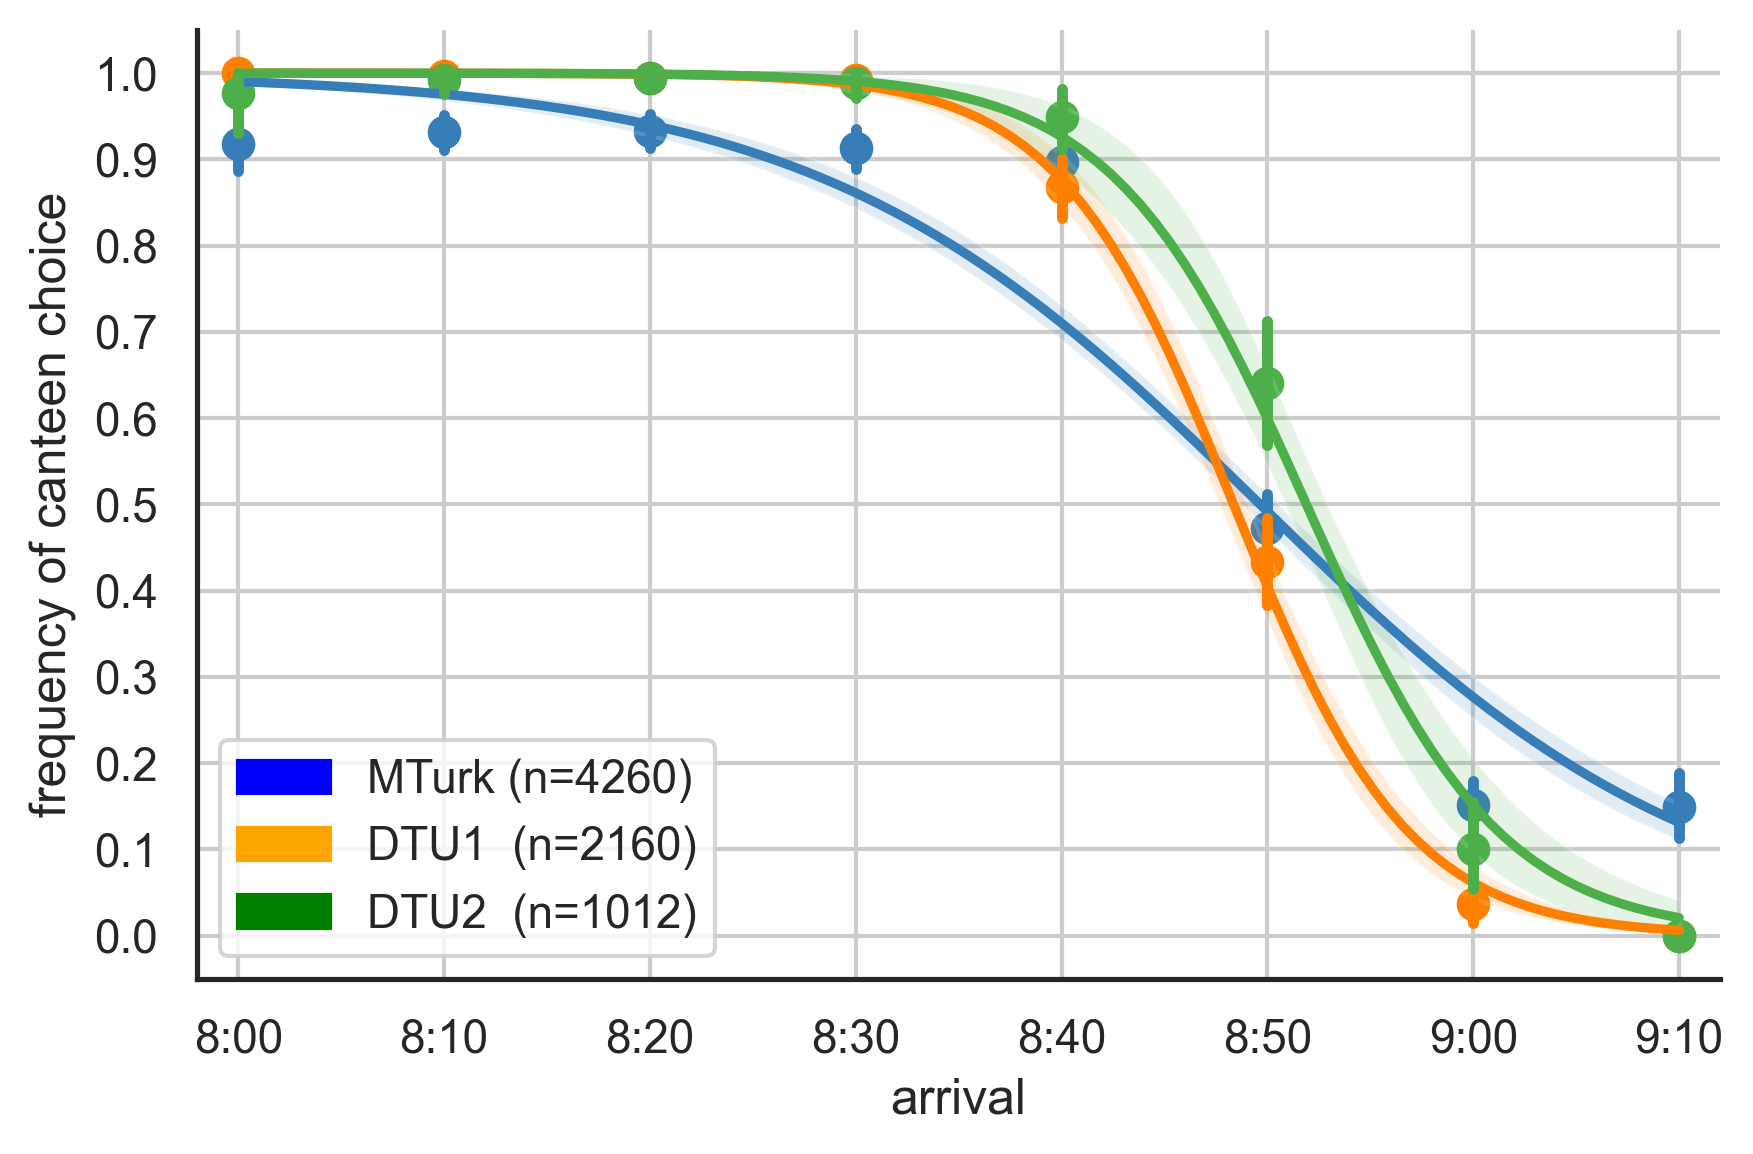
\includegraphics[width=0.8\linewidth]{fig1.png}
	\caption{Percentage of canteen choices as a function of arrival times. The colored lines are logistic regression lines with 95\% confidence intervals shown as translucent bands. Fitted parameters show significant differences in the slope and intercept between MTurk and DTU experiments ($p < .0001$).}
	\label{fig:1}
\end{figure}

To model the relationship between arrival time and the probability of choosing the canteen (choice), a logistic regression is performed in Fig.~\ref{fig:1}. The model computes a binomial model with bootstrapped confidence intervals (CI $=95\%$) for the estimated parameters. Bootstrapping is performed with $10.000$ iterations to ensure stable estimation of confidence intervals. MTurk participants in blue have a slightly more gradual decline of canteen choices for increasing arrival times. However, the point at which there is a $50\%$ probability of choosing the canteen or the office is close to $8{:}50$ in all three experiments (see further specfications in an additional mixed-effects regression analysis in Appendix~\ref{appendix:logistic}). Later, in Fig.~\ref{fig:indistinguish}, we make a combined regression analysis of all three experiments in order to understand the overall experimental results in terms of degrees of shared knowledge.

\begin{figure} %[t]
\centering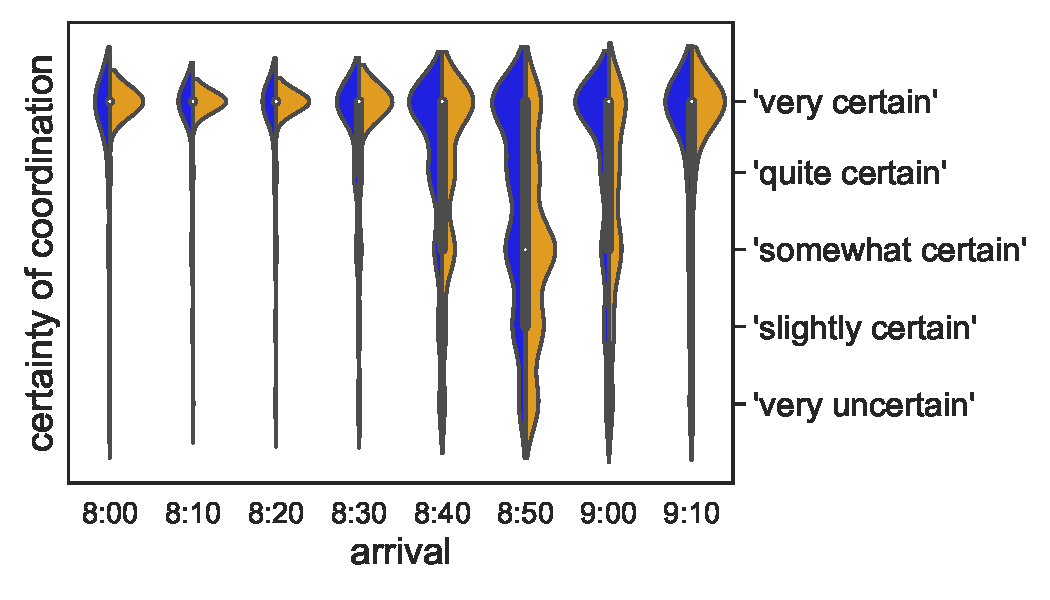
\includegraphics[width=0.8\linewidth]{fig2_certainties}
\caption{Violin plots of certainty estimates. In each round, participants were asked how certain they were of successful coordination with their colleague. Blue areas show the results from MTurk ($\text{n}=4260$) and orange areas show the results from DTU1 and DTU2 combined ($\text{n}=3172$). We predefined a five point likert scale of certainty estimates as: `very uncertain', `slightly certain, `somewhat certain', `quite certain', and `very certain', and translated them into the numerical values of probability estimates used in the payoff calculations (see Appendix~\ref{appendix:payoffs}). The white dots correspond to the median certainty estimate.}
\label{fig:certain}
\end{figure}

The violin plots in Fig.~\ref{fig:certain} show the distribution of certainty estimates for each arrival time. The DTU experiments are merged and compared with the MTurk experiment, as the differences between the two DTU experiments generally are smaller than their respective difference to the MTurk experiment. This is quantified in Table~\ref{table:1}, as the calculated average penalties per round are a direct consequence of the certainty estimates given by the participants. In general, however, Fig.~\ref{fig:certain} shows that it is exceedingly rare for any of the participants to consider it problematic to go to the canteen when arriving early. Arriving at $8{:}30$ or earlier is deemed sufficiently early to visit the canteen with very high confidence. %, and 
% \tobo{Isn't it more correct to say that that only happens at $8{:}30$ and that $8{:}40$, $8{:}50$ and $9{:}00$ all show some uncertainty? That's how it looks when I look at the violin plots. Only $8{:}30$ and earlier is really robust.} \re{agree. Someone please change to 8:30.} \tsn {Changed the text to 8:30, and adjusted text} 
%arriving at $9{:}00$ or later is deemed office time with high confidence, 
%arriving at $8{:}40$ is deemed either office or canteen with at least being ``somewhat certain''.
%and arriving at $8{:}50$ or $8{:}40$ is deemed either office or canteen with at least being ``somewhat certain''. 
The subtle differences in certainty estimates between MTurk participants and DTU students show that the latter tend to be slightly more certain that their co-players follow a similar strategy (higher certainty estimates for the early and late arrival times), and also that they are more aware of the danger of miscoordination (lower certainty estimates at $8{:}50$ and $9{:}00$). This is in particular the case for the DTU1 experiment that has the steepest profile. Being more certain that your co-players follow a similar strategy probably indicates that you believe such a strategy to be optimal. So, interestingly, the DTU1 participants are both the ones that appear to be most aware of the danger of miscoordination, and at the same time those who most firmly believe a cut-off strategy is optimal, i.e., believing that the risk of miscoordination is unavoidable. The differences between the three experiments are however still relatively minor. In the following we will combine data from all three experiments.

\begin{figure} %[!b]
\centering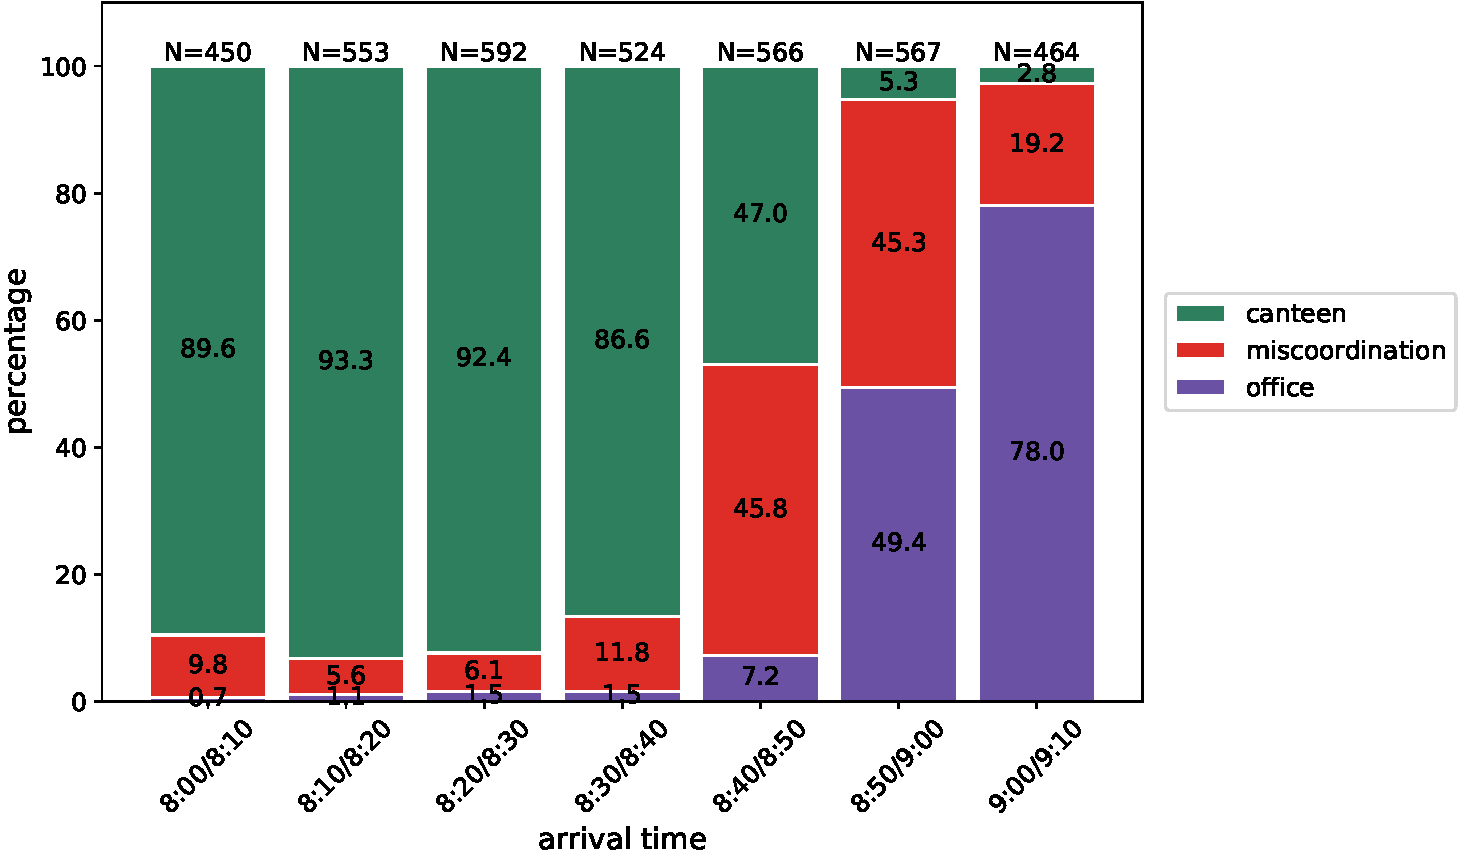
\includegraphics[width=0.8\linewidth]{fig3_miscoordinations}
\caption{Percentage of coordinations and miscoordinations as a function of arrival times. Green means coordinating into the canteen, purple means coordinating into the office, and red means miscoordination. We use the notation 8:00/8:10 to denote the union of the arrival pairs $(8{:}00,8{:}10)$ and $(8{:}10,8{:}00)$, i.e., the arrival time combinations where one of the players arrive at $8{:}00$ and the other at $8{:}10$. Miscoordinations approach $50\%$ at 8:40/8:50 and 8:50/9:00.}
\label{fig:miscoordinations}
\end{figure}

In Fig.~\ref{fig:miscoordinations}, we see the percentage of successful coordinations into the canteen or office (green or purple) together with the number of miscoordinations (red) as a function of all possible arrival time combinations. The figure shows that players are able to coordinate into the canteen more than 86\% of the time if both of them arrive before $8{:}50$. As soon as a pair has a player who arrives at $8{:}50$, however, the result changes drastically. Suddenly almost half of such pairs miscoordinate. As players experience harsh penalties for miscoordinating, one could perhaps expect to see a tendency of choosing office more often when arriving at 8:40 or 8:50 in subsequent rounds. That is, we might expect that players learn and converge to the all-office strategy in order to avoid miscoordination altogether. But this is not what we see.

\begin{figure} % [!t]
\centering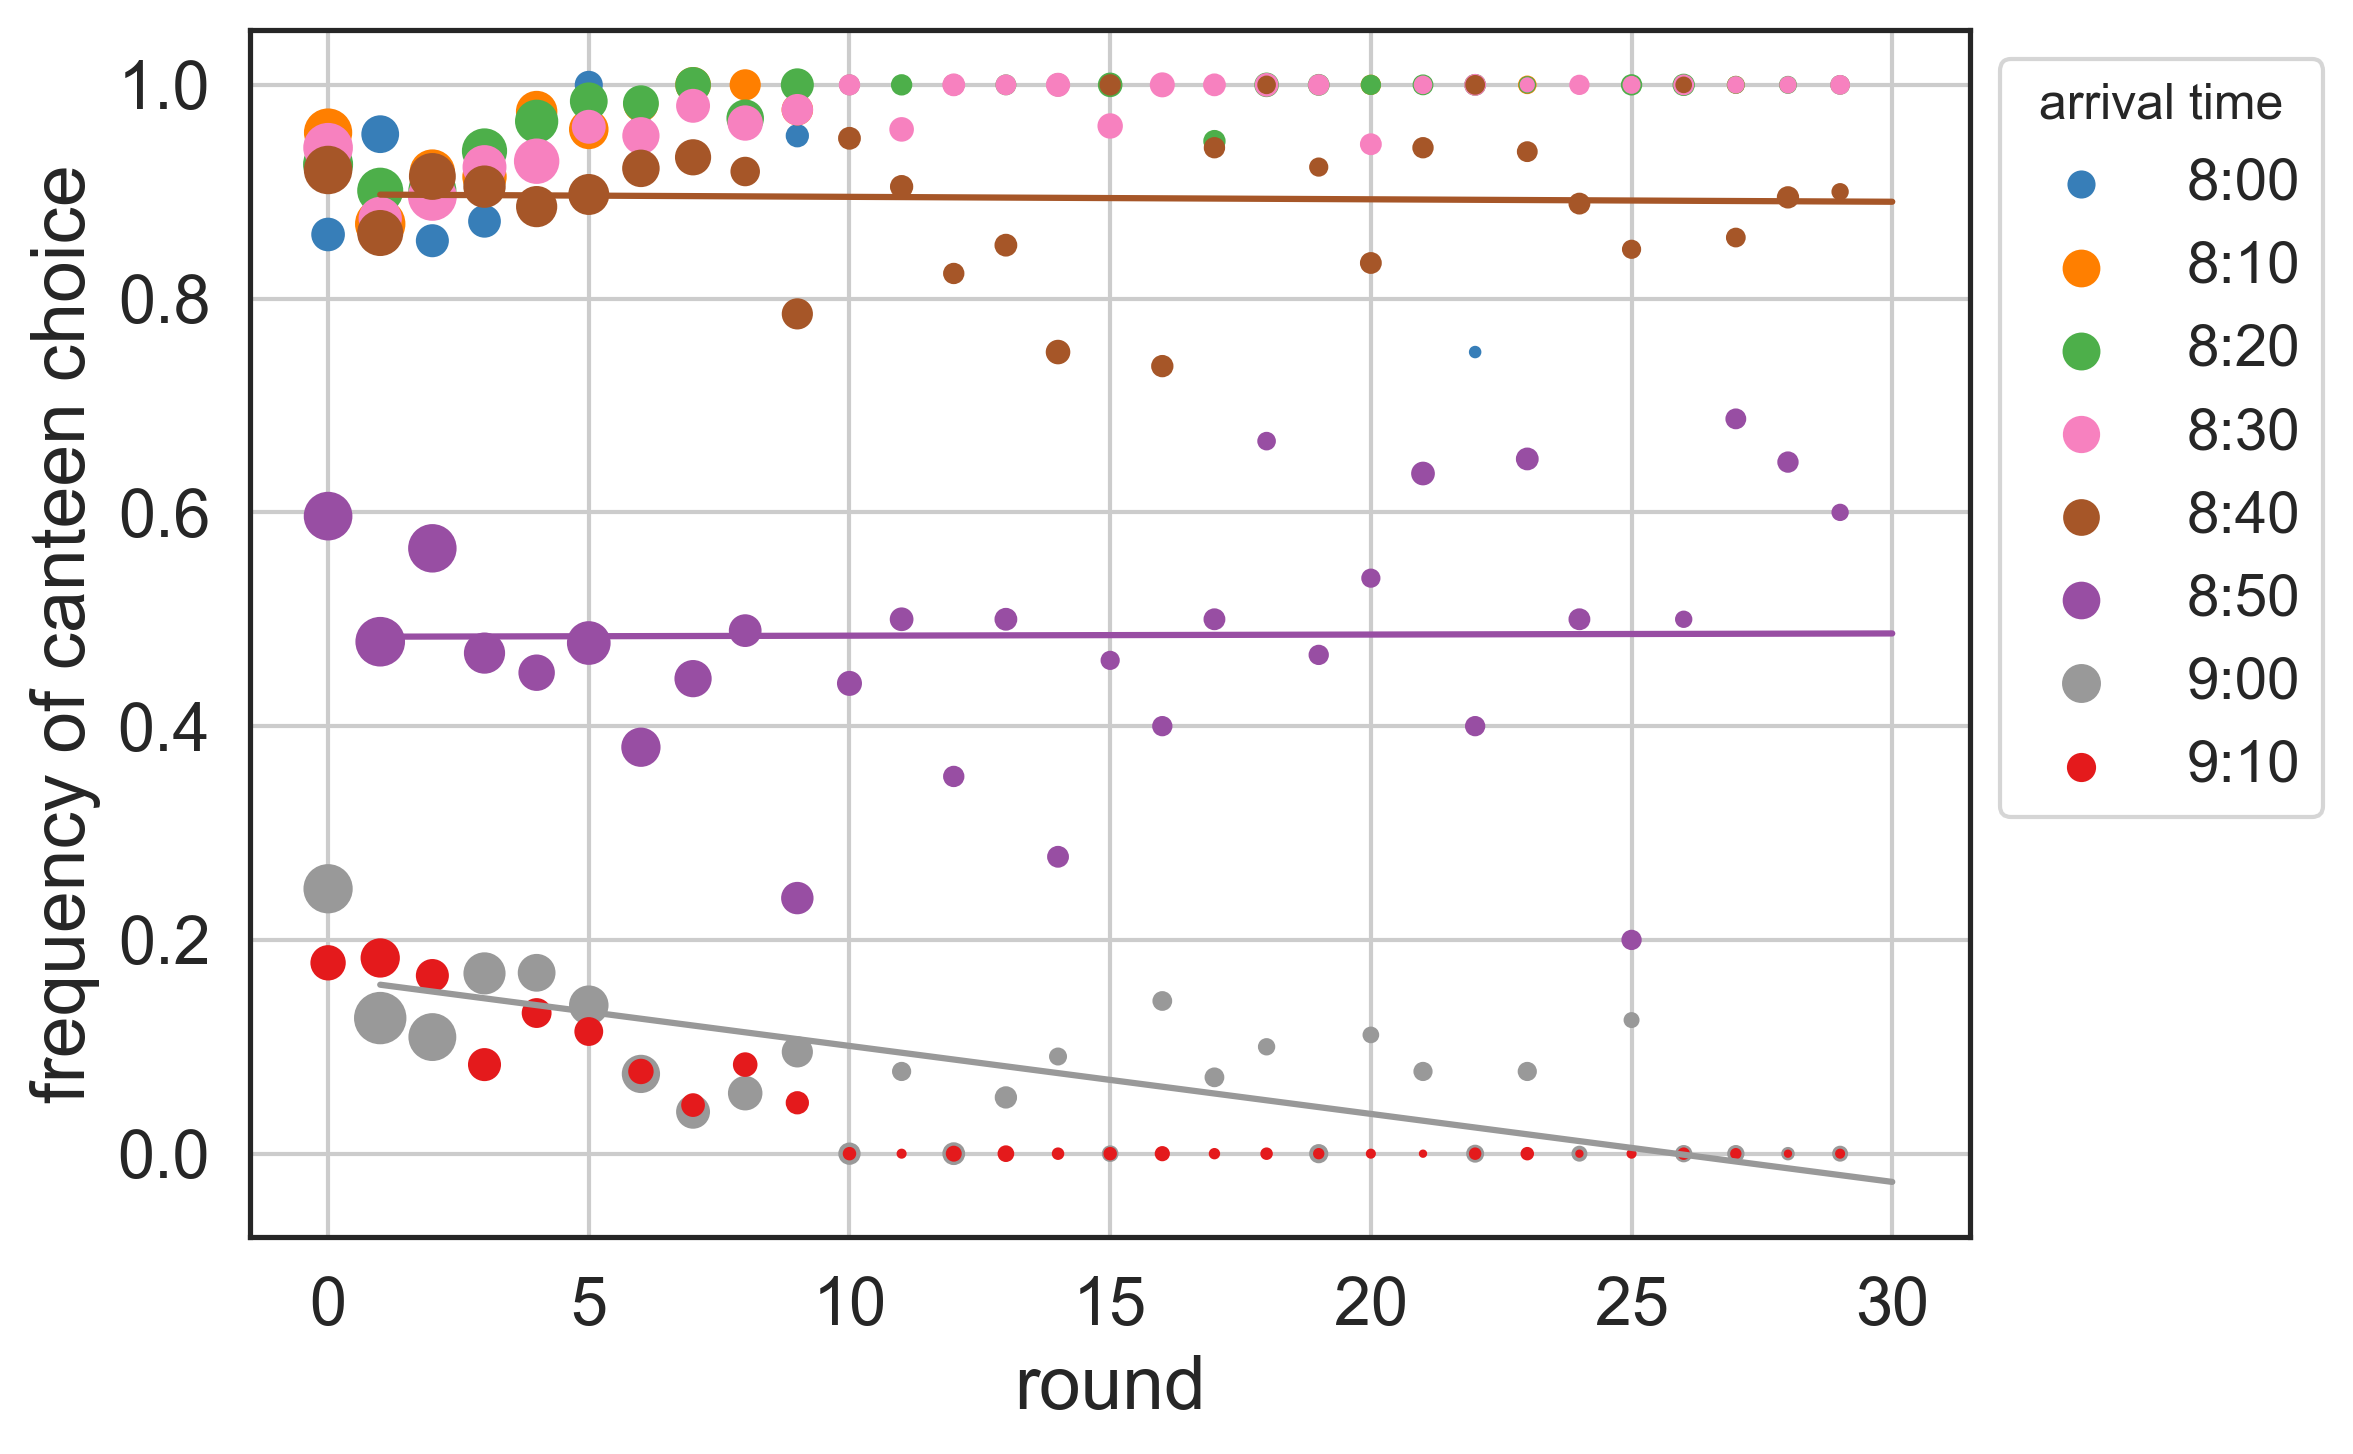
\includegraphics[width=0.8\linewidth]{fig4.png}
\caption{Mean frequencies of canteen choices for all possible arrival times as a function of the number of rounds played. The three fitted horizontal lines, corresponding to arrival times $8{:}40$, $8{:}50$, and $9{:}00$ respectively, represent weighted linear squares (WLS) with the weights chosen to be the square root of the number of data points constituting the mean frequencies for each round, also shown by dot size.}
\label{timeseries}
\end{figure}
Fig.~\ref{timeseries} shows the mean frequency of canteen choices as a function of rounds played for all three experiments. Each color corresponds to a certain arrival time. Clearly, the only arrival times that do not converge towards either the canteen or the office are the arrival times of $8{:}40$ and $8{:}50$, with the former fluctuating around $90\%$ canteen choices and the latter fluctuating around $50\%$ canteen choices. This indicates that there is no behavioral change during the game. Participants arriving at $8{:}40$ or $8{:}50$ do not feel incentivized to change their behavior significantly in subsequent rounds, even though there is a high risk of miscoordination. This is not to say that participants do not learn that canteen choices at $8{:}40$ or $8{:}50$ are dangerous. Partitioning the data from Fig.~\ref{fig:1} into two bins, corresponding to pairs having had no miscoordination and pairs having had one or more miscoordinations (see the supplementary data analysis in Appendix~\ref{app:supplementary-data-analysis}), shows somewhat decreasing certainty estimates around the critical arrival times. However, this does not affect their actual choices. MTurk participants do choose the canteen a little less often after a miscoordination (see Fig.~\ref{fig:certainties} in the appendix), but this does not translate into better payoffs as later miscoordinations just move to earlier arrival times. So even though participants learn that their choices are risky, they do not see any way to improve their strategy (at least not in the short term). Specifically, they never converge to the optimal all-office strategy, and also not to the alternative canteen-before-9 strategy (cf.\ Theorem~\ref{theorem:all-office-or-cut-off} in Appendix~\ref{appendix:formal}). This apparent lack of behavioral change in higher-order social reasoning games was also identified by Verbrugge~\cite{verbrugge2008learning}. 

\begin{figure} %[t]
  \centering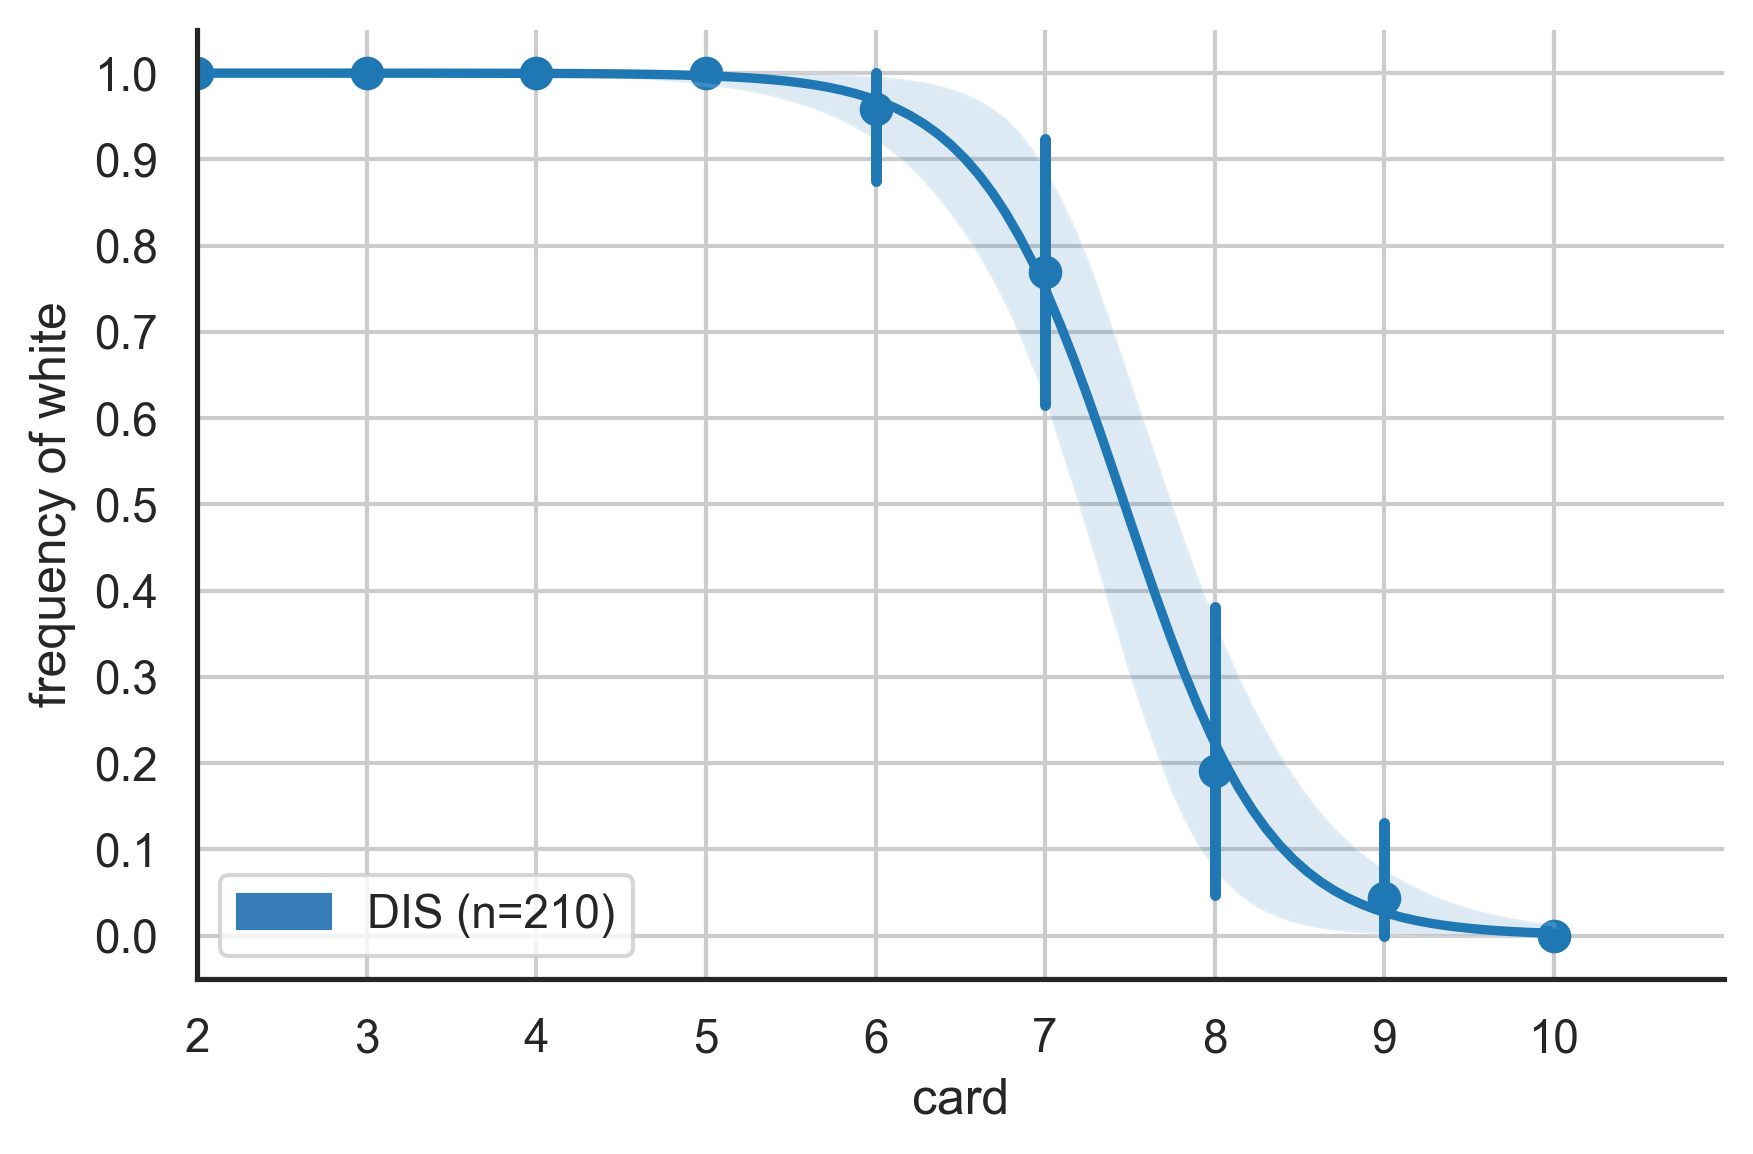
\includegraphics[width=0.6\linewidth]{fig5_DIS.png}
  \caption{Logistic regression of the relationship between card number and choice of a white stone in the qualitative experiment at DIS. The resulting curve shows a very similar overall trend as in the main experiments shown in Fig.~\ref{fig:1}.} 
  \label{fig:dis} 
  \end{figure}  
Fig.~\ref{fig:dis} shows the results for the alternative version of the game conducted at DIS, where players are dealt cards with numbers from 2 to 9, and choose either a black or a white stones (cf.\ Section~\ref{sect:experimental_design}). Choosing a white stone corresponds to choosing office in the original version of the game, and getting a card with the number $n$ corresponds to arriving at $9{:}00+00{:}10(n-9)$ in the original game. So e.g.\ receiving card 7 correponds to arriving at $8{:}40$, receiving card 8 corresponds to arriving at $8{:}50$, and receiving card 9 corresponds to arriving at $9{:}00$. The results in Fig.~\ref{fig:dis} are very similar to the results of the original version of the game, Fig.~\ref{fig:1}. The curve has the same shape, and with a slope that is most similar to the DTU experiments (which makes sense, as here the participants are also students in computer science and AI). The choices at 6 ($8{:}30$) are more than $90\%$ white (canteen), and the choices at 9 ($9{:}00$) are more than $90\%$ black (office), similar to the DTU1 experiments. The choices at 8 ($8{:}50$) are around $20\%$ white (canteen), which is lower than for any of the original experiments, suggesting a potentially better understanding of the risk of miscoordination. Alternatively, it might be due to the fact that in this version of the game, miscoordination leads to immediately losing all earnings, so the penalty of miscoordination is even clearer and higher in this version of the game (this was a deliberate choice in our game design, in order to make sure that the observed results of the original game were not due to unawareness of the high penalty of miscoordination).% The certainty estimates in this version of the game are also very similar to the original version, see Figure
%~zref{fig:dis_certainties} 
%@@@fix this@@@ in  \nameref{supplementary_material}.
%The only difference is that the participants in the alternative version of the game are more likely to choose white stones (canteen) when receiving cards with numbers 8 and 9, compared to the original version of the game. This is likely due to the higher payoff for choosing white stones when receiving cards with numbers 8 and 9 in the alternative version of the game, compared to the original version of the game.
%However, in the alternative version, participants are more likely to choose white stones (choosing canteen) when receiving a card with number 8 (when arriving at $8{:}50$)   
%These show behavior similar to our canteen version, although with more choosing white (similar to canteen) at 8 (similar to 8:50) than in the canteen game. We nevertheless see the same drastic increase in "white" choices in the following numbers.

The DIS classroom experiment was followed by a number of qualitative interviews with the students, divided into groups of 4.  These confirmed that the players considered the rules to be common knowledge. 
% about the rules.  
%had common knowledge about the rules, as well as their intuitive sense of white becoming an increasingly safe strategy when the card numbers decrease. 
When asked about the existence of safe strategies guaranteeing coordination (always choosing the same stone), 
most players expressed the false belief that a cut-off strategy existed that would guarantee coordination on white stones for sufficiently low numbers (which we proved false in footnote~\ref{footnote:no-cutoff}). Most players believed that the cut-off would be around 6 or 7,  
%a cut-off strategy of around 6 or 7 was safe in order to coordinate, 
although some realized during the interview that such a  strategy can never guarantee coordination. Only one student was skeptical about the existence of a safe strategy for coordinating on white from the very beginning of the interview. 




\section{Discussion}\label{discussion}
Let us try to analyse the experimental results in terms of the depth of knowledge of the participants. The highest payoff is achieved when successfully coordinating into the canteen before 9:00. With the aim of achieving the highest possible payoff, each participant can be expected to consider her own arrival time and try to assess whether there is still time to meet in the canteen. When a participant arrives strictly before 9:00, i.e.\ at $8{:}50$ or earlier, she has private knowledge that she arrives sufficiently early to go to the canteen. If participants only make choices based on their private knowledge, we should then expect participants to always go to the canteen at $8{:}50$. This is not what we see, cf.\ Fig.~\ref{fig:1}. Thus, other considerations in addition to the player's private knowledge must play a role in their decision making.

When both participants know they arrived before 9:00, they have shared knowledge of having arrived in time for going to the canteen. This happens for any arrival pair $(t_1,t_2)$ with $t_i \leq 8{:}50$, $i=1,2$ (where an \emph{arrival pair} $(t_1,t_2)$ denotes that player $1$ arrives at time $t_1$ and player $2$ at time $t_2$, see Appendix~\ref{appendix:formal} for further details). Note that for an arrival pair $(8{:}50,8{:}40)$, there is shared knowledge of there being sufficient time to go to the canteen, but only player $2$ knows this fact: Player $2$ knows that also player $1$ must have arrived before 9{:}00, but player $1$ doesn't know this about player $2$. In other words, when a player arrives at $8{:}50$, that player considers it possible that there is shared knowledge of there being sufficient time for a cup of coffee in the canteen, but only if arriving at $8{:}40$ or before will that player \emph{know} there to be shared knowledge (to depth 1). When arriving at $8{:}30$ or before, the player additionally knows there to be shared knowledge to depth 2. We illustrate this in Fig.~\ref{fig:indistinguish}. Note that in general, if a player arrives at time $8{:}50-0{:}10n$, $n>0$, then that player knows that there is $n$th-order shared knowledge, but the player doesn't know there to be $(n+1)$st-order shared knowledge. This follows a similar pattern as the mountain trekking example, except here the depth of shared knowledge is determined by how early ahead of 9:00 the agents arrive, rather than how many messages have successfully been delivered. No number of messages was sufficient to achieve common knowledge in the mountain trekking example. We similarly get that no arrival time is sufficiently early to establish common knowledge of having sufficient time to meet for coffeee in the canteen. 

\begin{figure} %[t]
\[
  \begin{tikzpicture}[align=left,xscale=0.9]
   \node[anchor=west] at (-1.0,-2.5) {players' \\ knowledge level}; %of\\ sufficient time for canteen:};
   \node[anchor=west,red] at (-1.0,0.9) {arrival time \\ player 1:};
   \node[anchor=west,mygreen] at (-1.0,-1) {arrival time \\ player 2:};
   \node[red] (n1820) at (3,1) {8{:}20};
   \node[mygreen] (n2820) at (3,-1) {8{:}20};
    \node[red] (n1830) at (5,1) {8{:}30};
   \node[mygreen] (n2830) at (5,-1) {8{:}30};
   \draw[-] (n1820) to (n2830);
   \draw[-] (n2820) to (n1830);
  \draw[dashed] (4,-3) to (4,1.5);
    \node[red] (n1840) at (7,1) {8{:}40};
   \node[mygreen] (n2840) at (7,-1) {8{:}40};
    \node[red] (n1850) at (9,1) {8{:}50};
   \node[mygreen] (n2850) at (9,-1) {8{:}50};
     \draw[-] (n2840) to (n1850);
   \draw[-] (n1840) to (n2850);
   \draw[-] (n1830) to (n2840);
   \draw[-] (n2830) to (n1840);
  \draw[dashed] (6,1.5) to (6,-3);
  \draw[dashed] (8,1.5) to (8,-3);
     \node[red] (n1900) at (11,1) {9{:}00};
   \node[mygreen] (n2900) at (11,-1) {9{:}00};
    \node[red] (n1910) at (13,1) {9{:}10};
   \node[mygreen] (n2910) at (13,-1) {9{:}10};
     \draw[-] (n2850) to (n1900);
   \draw[-] (n1850) to (n2900);
   \draw[-] (n1900) to (n2910);
   \draw[-] (n2900) to (n1910);
  \draw[dashed] (12,1.5) to (12,-3);
  \draw[dashed] (10,1.5) to (10,-3);
  \node at (13,-2.5) {none};
  \node at (11,-2.5) {none};
  \node at (9,-2.5) {private};
  \node at (7,-2.5) {shared\\ depth 1};
  \node at (5,-2.5) {shared\\ depth 2};
 \node at (3,-2.5) {shared\\ depth 3};
 \node at (7.8,0)
 	{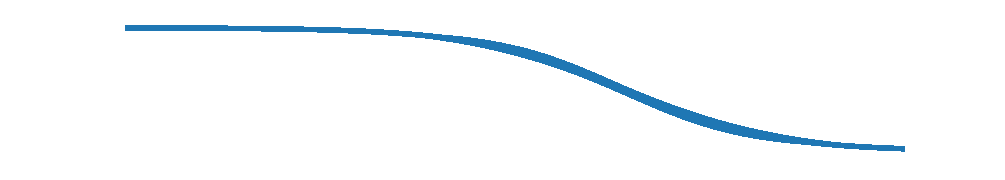
\includegraphics[scale=.75]{fig5_logit_all}};
  \end{tikzpicture}
  \]
  \caption{The solid diagonal lines express indistinguishability for the players, e.g.\ the arrival time $8{:}40$ for player $1$ has a line to both of the arrival times $8{:}30$ and $8{:}50$ for player $2$, since these are the two arrival times for player $2$ that player $1$ will consider possible when herself arriving at $8{:}40$. Below each possible arrival time, we have marked the highest level of knowledge of there being sufficient time to go to the canteen, e.g.\ when arriving at $8{:}40$, there is shared knowledge to depth 1 of this fact, but not shared knowledge to depth $2$. In blue, a binary logistic regression model was used to predict the probability of a participant going to the canteen (upper limit) or to the office (lower limit) at the shown arrival times. The width of the regression line indicates the 95\% confidence interval using 10.000 bootstrapped resamples of all choices in all three experiments ($\text{n}=7432$).
  }\label{fig:indistinguish}
\end{figure}
The participants seem to clearly be able to distinguish between private and shared knowledge, which is supported by their significantly different choices at $8{:}50$ and $8{:}40$ (see again Fig.~\ref{fig:indistinguish}). However, it is less clear whether they are able to robustly distinguish different levels of shared knowledge, and whether they are able to distinguish that from common knowledge. Indeed, most participants relatively robustly choose the canteen at $8{:}40$ and any time before that, despite the difference in depth of shared knowledge in those possible arrival times. The certainty estimates are however slowly decreasing from $8{:}10$ to $8{:}50$ in all three experiments (see Fig.~\ref{fig:certain}), showing that the participants are not completely ignorant to the differences. This could suggest that many participants believe that it is less safe to go to the canteen based on $n$th-order shared knowledge than $(n+1)$st-order shared knowledge. Very few seem to draw the conclusion that it is never safe to go to the canteen, or, if they do, they at least don't expect the other player to be able to draw the same conclusion. 

Why do participants not regard earlier office choices as viable options? Why do participants not continue their train of thought and deduce that when $8{:}50$ turns out to be unsafe, $8{:}40$ will become unsafe as well, which means that $8{:}30$ will also be unsafe, etc.? One reason may be that the all-office strategy is cognitively difficult to comprehend given the  limited  ability of humans to take the perspective of each other recursively. 
%~\footnote{We have played the Canteen Dilemma with many people, and even when explaining to them that there is no safe cut-off strategy (except the all-office strategy), many of them simply do not accept the argument, instead insisting that there \emph{must} exist a cut-off time that is sufficiently early.} 
One might also speculate that the players suffer from a 
computational overload from the complexity of the game's rules and payoff structure. While this may be a problem, we do not think it has much significance for the following reasons. If computational overload was sufficient to distract our participants, we might expect more varied suboptimal choices. While we do see some bluntly irrational choices of canteen at 9:00 (given the rules and payoff structure), the vast majority choose office at 9:00 and 9:10, and canteen at earlier arrival times, with many still choosing office at 8:50. Besides this, we see participants be much less certain of their canteen choices at 8:50 or 8:40 than at earlier arrival times. 

Another reason for not considering earlier office choices as viable may be that while the optimality of an all-office strategy are understood, the participants do not believe that this is common knowledge, and hence they do not rely on the other participants to choose the same strategy. That is, they either think their co-player does not realize there is no safe cut-off, or that their co-player thinks this about them, and so on. In this way, the strategic reasoning involved becomes akin to the Keynesian beauty contest~\cite{keynes1936general,nagel1995unraveling}. Under this assumption, we should not necessarily expect participants to play an all-office strategy, since that is only proven optimal when assuming there to be common knowledge of perfect rationality (see Appendix~\ref{appendix:formal}). A possible alternative strategy may be the following mixed strategy: 1) always go to the canteen before $8{:}50$, 2) always go to the office after $8{:}50$, and 3) go to the canteen with probability $0.5$ at $8{:}50$. If both players follow this strategy, the arrival time combinations $8{:}40/8{:}50$ and $8{:}50/9{:}00$ will then coordinate $50\%$ of the time, matching well with what we observe in Fig.~\ref{fig:miscoordinations}. If this is the strategy followed, and if players assume their co-players to follow the same strategy, they should also be aware of the $50\%$ probability of miscoordination at $8{:}50$. In Fig.~\ref{fig:certain}, we indeed see a much lower coordination certainty estimate at 8:50. However, if players were indeed playing this strategy and assuming their co-players to do the same, their certainty estimates ought to be even much lower at 8{:}50. % TODO: TSN: This wording is a bit confusing to me
 These certainty estimates also ought to be lower if we assume that players are aware of the possibility of their co-players not being perfectly rational and their chosen strategy hence to be somewhat unpredictable. 


\begin{figure} %[h]
\centering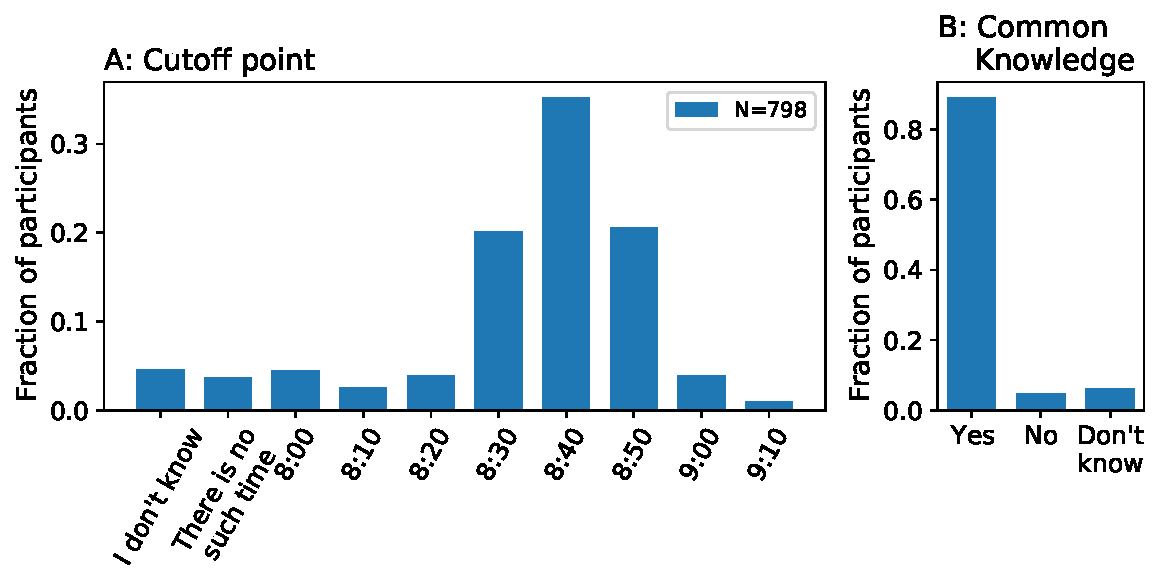
\includegraphics[width=1\linewidth]{fig6_cutoff}
\caption{A) Frequencies of answers to the question: ``Imagine you could have agreed beforehand with your colleague about a point in time where it is safe to go to the canteen. What time would that be?'' Due to the pragmatics of language, we assume that an answer like 8:30 entails the belief that all earlier arrival times would also be deemed safe. B) Frequencies of answers to the question: ``Imagine you arrive at 8:10. Is it common knowledge between you and your colleague that it is safe to go to the canteen, that is, that you both arrived before 9:00?''}
\label{fig:cutoff answers} % silly name!
\end{figure}
Probing theses questions further, we asked participants the following post-game question:
\begin{quote}
\indent
``Imagine you could have agreed beforehand with your colleague about a point in time where it is safe to go to the canteen. What time would that be?'' \textit{('I don't know', 'There is no such time', 8:00, 8:10, 8:20, 8:30, 8:40, 8:50, 9:00, 9:10)}
\end{quote}
The results in Fig.~\ref{fig:cutoff answers}A show that most answers range from 8:30 to 8:50 (approximately $75\%$ of all answers), giving support to the verdict that participants are not able to continue taking the perspective of each other recursively, or at least that they believe that shared knowledge of some modest finite depth is sufficient for the canteen choice to be safe. Rather, they stop after one or two, possibly three, iterations, thus believing that as long as they arrive sufficiently early, they can be sure to coordinate safely in the canteen. Notice that the correct answer, ``there is no such time'', is chosen by less than $4\%$ of all participants. The interviews with students in the DIS experiment indicates the same. One student claims for example that ``(from) two to five, there is no risk involved''. This also reflected in the results, as Fig.~\ref{fig:dis} shows, no students plays black (equivalent to an `office' choice) for numbers 5 and below. One interview from the DIS experiment also ends with a student asking ``Did you find an optimal number?''. 

The answers to the post-game question above, as well as the DIS interviews, indicates that the prevalence of canteen choices is not due to uncertainty about the rationality of other players, but instead due to a more immediately available belief, that there is a point where canteen choices (or white stones in the DIS experiment) can be played without the risk of miscoordination. In reality, they would need common knowledge in order for the canteen choice to be without risk, and the players seem to behave as if they have such common knowledge. 
% supporting the conjecture stated in the introduction that moderate depths of shared knowledge become effectively indistinguishable from common knowledge.\tobo{Maybe this is one of the places where we could consider to moderate the claim. The question they are asked is not explicitly about common knowledge, and it is not about common knowledge as achieved via public announcements. The question doesn't in itself prove that they can't distinguish shared knowledge of moderate depth from common knowledge. But it shows that they will strategically behave as if they had common knowledge, and will not realise that the unsafety argument can be iterated. So they get "tricked" to believe they can safely coordinate, which means that in some sense their beliefs and actions compare to the common knowledge setting, but I'm not sure we can *strictly* claim the shared knowledge is indistinguishable from common knowledge?}  \tsn {Good point, and I'm not sure, difficult discussion. We want to say that our participants behavior is coextensive with common knowledge behavior. Not sure how to put it. It might be good for various reasons to not focus too much on mental states in general, and look at behavior, but this research field is generally not so behaviorist.} \re{agree as well. We can't really say anything about their understanding of common knowledge from this question. Proposal: remove text starting from ", supporting the conjecture".} \tsn {Support as well.} 
Participants might of course not necessarily have a precise idea of the technical notion of common knowledge and how it differs from $n$th-order shared knowledge, but as discussed in the introduction, there is actually quite a number of studies demonstrating that humans have adapted to recognize common knowledge and making distinct strategic choices depending on whether there is common, shared or private knowledge---at least in cases where the difference between these states of knowledge is relatively clear (for instance when the common knowledge situation is achieved via a public announcement). In our experiments, we see the player behavior stabilizing already at relatively modest depths of shared knowledge, both in terms of action choices and certainty estimates. We also see that player behavior does not match what we would expect to see if they only believed to have $n$th-order shared knowledge, but instead matches what we would expect to see if they indeed wrongly inferred common knowledge. 

To specifically address the issue of whether they wrongly infer common knowledge, we asked a final post-game question:

\begin{quote}
\indent
``Imagine you arrive at $8{:}10$ am. Is it common knowledge between you and your colleague that it is safe to go to the canteen, that is, you both arrived before $9{:}00$ am?''. \textit{(`Yes', `No', `Don't know')}
\end{quote}

\noindent
This question inquires about participants' understanding of the term `common knowledge', and how it applies to the given situation. In Fig.~\ref{fig:cutoff answers}B, the results show that $89\%$ of all participants responded that it was common knowledge that both players arrived before $9{:}00$ when they themselves had arrived at $8{:}10$. The answers may signify that indeed they believe there to be common knowledge in the strict technical (logical) sense. But of course the answers could also pertain to the everyday linguistic usage of the term `common knowledge', which is less strict.







%\subsection{Ecological Validity} \label{ecovalid}
%A relevant discussion relates to how close our experimental setup is to real-world scenarios. We identify a few possible issues here. First, we might ask if participants had a natural preference for canteen outside of the game, which caused them to act sub-optimally in the game. This we find unlikely to be the case. The Canteen Dilemma was evolved from an earlier, purely abstract, version of the game. In this earlier version, the two players each privately received a number in the interval 1-10 and was being told that the other player got a number either one higher or one lower. The players could then choose between two options, A and B. If both chose A and both numbers were strictly below 10, the players would get the highest payoff. If both chose B, they would still get a positive, though much lower, payoff. In all other cases they would lose all their earlier payoffs and the game would end. In this version, the optimal strategy is to always play B (corresponding to the office-only strategy). The only incentive to play A would be to get the higher payoff, but as in the Canteen Dilemma, any strategy which involves A (corresponding to the canteen-choice) will include risk of miscoordination. \st{it is never safe to play A since there will never be common knowledge that both numbers are below 10.} This version of the game \st{The fact that there can never be common knowledge that both numbers are below 10} is known as the consecutive number riddle~\cite{van2015one} or the Conway paradox~\cite{van1980conway}, from where we originally found inspiration for our game. In the original abstract version of the game, we observed the exact same player behavior as in the Canteen Dilemma. Due to the potential opaqueness of the relatively abstract formulation of the original game, we decided for the canteen version, which was believed to be more immediately graspable and potentially more ecologically valid.  \add{We also conducted a followup experiment using this formulation, and found similar results in player behavior. This was corroborated by interviewing the participants after the experiment, which revealed a general belief that some cutoff point or strategy is possible, which involve playing A but does not risk miscoordination. To summarize, we do not believe that players choosing canteen over office reflects a natural propensity towards coffee. }
%We started out with informal testing on people using integer values instead of arrival times, and asking them to coordinate if both got a number below some integer (the consecutive number game \ \citet{van1980conway,van2015one}). We decided against this exactly for reasons of ecological validity, since the abstraction made the game unnecessarily opaque. TODO: Expand this?


%Second, we can ask if situations arise in the wild where there is only shared knowledge to some degree but not common knowledge. \st{---and where we would have a tendency to assume common knowledge with potentially large negative consequences}. We will argue that such situations are quite common, \add{especially online.}  \tsn{Vi har måske et problem her, fordi vi beskriver mangel på common knowledge som de tilfælde hvor viden om P ikke er delt af alle (nogle hører ikke efter, eller email ikke når frem). Men det er de simple og lette at forstå tilfælde. Vi vil gerne beskrive den komplekse situation hvor alle ved P, (og måske alle ved at alle ved det etc) men at det stadig ikke er common knowledge. Det er måske mere sandsynligt, hvis vi får en fællesbesked på et medie, som alle læser, men hvor kun nogle svarer. Generelt er problemet nok mere realistisk (indenfor eco. valid.) indenfor online communication, hvilket også er forklaring for hvorfor face-to-face møder er essentielle indenfor vigtige beslutninger} 

%\add{Public broadcasting of messages, e.g.\ instructions given in a classroom to a class of pupils or an email sent by the department head to everybody in a university department, will in practice not necessarily lead to common knowledge. Some of the pupils might not be paying attention at the moment, or have misinterpreted the message. Even if they acknowledge it, the same arguement repeats, as the students cannot be certain their acknowledgements were properly received. The error rate for communication in such public broadcasting scenarios is relatively low however. It is worse for online, or written communication. Here it is much less clear if everyone have checked their email, or if the email was correctly delivered. In fact, we know that contrary to face-to-face communication, the messages of emails are rarely read instantly by recipients. So, you cannot cannot be certain everyone have read your email. And likewise, even if everyone sends an acknowledgment email, they cannot be certain that you have read it. }

%\st{Public broadcasting of messages, e.g. instructions given in a classroom to a class of pupils or an email sent by the department head to everybody in a university department, will in practice not necessarily lead to common knowledge. Some of the pupils might not be paying attention at the moment, and some of the department employees might not have checked their email, or it might have ended up in their spam filter. Suppose that the message was regarding to all meet at a certain place at a certain time. Can we then be sure that everyone will meet at that place at that time?  Obviously, no.  Then the reply might be that we can just ask everybody to confirm that they received the message, e.g.the school teacher might ask the children to confirm that they heard the message. Well, yes, but then the same argument repeats for the confirmation messages: the recipient of the confirmations might not receive all of them or might briefly not pay attention. }

%Now, this generalizes to all social situations and while it does not mean that we do not often obtain common knowledge, it means that we sometimes do not, and end in epistemic situations akin to the canteen dilemma. No amount of confirmations can guarantee common knowledge, and the risk of miscoordination will still be there. However, our hypothesis is that no matter how large the penalty is for miscoordination, when the level of shared knowledge has become sufficiently high, we will act as if common knowledge has already been achieved, it is at least being confirmed in the setting of the canteen dilemma.   . %And probably in most real-life cases the penalty for falsely assuming common knowledge might be somewhat lower than in the canteen dilemma, e.g.\ it might just be that someone doesn't show up for the event that the original message concerned. 



%We also note that in most everyday situations, the penalty for confusing shared knowledge with common knowledge is probably much lower than in our game. If it is for instance a group of pupils who are asked to meet at a certain time and place to get on the bus home from a school trip, confusing shared knowledge with common knowledge is not likely to be a big problem. It just means that the children will meet at the designated time and place despite not having common knowledge that all other children will also be there. In this case, the confusion of shared knowledge with common knowledge might even be helpful, since it allows coordination despite the lack of common knowledge. But this only happens because there is no large penalty if coordination fails. Even if one child eventually doesn't show up, it is probably better for all the other children to arrive anyway rather than not going due to the risk of someone else not showing up. In certain cases, it could however be different. \tsn{Måske skal vi ændre/slette eks. ovenfor?} \add{ Say you write an email to people saying you will buy an expensive plane ticket for them for a trip, unless they cannot go. If a person does not answer, you cannot be certain if they in fact wont show up, but just have not read your email, resulting in you buying a ticket for nothing. So, you decide to write that you only buy tickets for those who answer your email. Even if they acknowledge your email, and you read it, they might still not be certain you have read the email in time, so they buy a plane-ticket for themselves, leaving you both buying tickets. And even if you acknowledge their acknowledgement, you cannot be certain they read it, in which case you know they will buy a plane ticket. This may you to not buy a ticket for them, but where they don't do so either, since they in fact did read your acknowledgment. We may intuivetively avoid such cases where miscoordination is costly, either by making rules such that no coordination is necessary (everyone fends for themselves) or by making agreements face-to-face.  Our experiments show however that when we are in such situations, we do not seem to understand the impossibility of coordination, even after multiple miscoordinations. This is not to say that we should not try to coordinate, but that we should consider the risks of miscoordination if we coordinate in writing } \tsn{Det er måske dumt at have noget normativt med her? Det er et forsøg på at bygge ovenpå eco. validity pointen}
%The problem of these scenarios is two fold. First, such scenarios are difficult to grasp, as our experiments have shown, making it harder to see the possibility of miscordination. Second, our intuition concerning such scenarios are likely determined by the possibility of faulty communication and the consequences of miscoordination. That is, we might not grasp the chance of miscoordination if its consequences are sufficiently small.

%In general, if a group tries to coordinate a public demonstration, a dangerous emergency rescue or coordinate to all write letters of complaint, they might suffer a high penalty if a sufficiently high number of group members end up not participating. In this case, confusing shared knowledge with common knowledge can be critical, and it can be critical to be in a situation where common knowledge cannot be achieved (e.g.\ if trying to coordinate via posts on social media or trying to shout through the walls of a burning building). 
% go home from a school trip 
%For instance, in the example above it might just be that someone doesn't show up at the agreed place and time, and though this could lead to a high penalty for those who don't show up, it might not lead to a high penalty for everybody involved in the coordination effort. However, there \emph{could} be such a high joint penalty, e.g.\ if the class is supposed to meet for the bus to get home from a trip to a museum, and then...
%this might not lead to a high penalty for everybody involved in the coordination task. 


%Still, probably in most real-world scenarios, the penalty for miscoordination is lower than in our canteen dilemma. However, if that is indeed the case, then we should expect humans to pay \emph{more} attention to the potential confusion of shared knowledge for common knowledge in the game than in the wild.  In other words, if participants do not pay attention to it in our game, we should not expect them to be more aware of it in the wild.

%We might have evolved to do our best to avoid such situations, due to the complexity involved. This might explain why we do not identify it everywhere in our daily life. But it is unlikely that we can categorically deny that such situations arise. \st{and when they do, some might implicitly assume common knowledge to be present, while others, on a lower order of shared knowledge might not.} This results in miscoordination which people cannot predict, and possibly not even post-hoc understand. 


\section{Conclusion and future work} \label{S:conclusion}
We developed a new coordination game, the \emph{Canteen Dilemma}, to examine higher-order social reasoning in humans. Our experimental results %suggest that high levels of recursive perspective-taking are cognitively unavailable to the vast majority of players of the game. We see a
indicate a substantial degree of miscoordination, even in scenarios where coordination \emph{is} achievable (albeit only for the second-highest payoff). This miscoordination appears to stem from what we term the ``curse of shared knowledge'': an illusion of common knowledge in situations where only shared knowledge exists, and only to a limited depth. While the game results alone do not conclusively demonstrate that this illusion of common knowledge occurs, they show that players behave as though they have common knowledge. Moreover, variations to the game and responses to post-game questions strongly suggest the presence of this illusion. For instance, an overwhelming majority of participants report having common knowledge about the safety of arriving at the canteen at $8{:}10$ (Fig.~\ref{fig:cutoff answers}B). Additionally, qualitative interviews following the DIS classroom experiment further supported this interpretation. 

While we cannot claim to have definitely proven the existence of a 'curse of shared knowledge', our experiments support it as a plausible conjecture that warrents further investigation. This result is somewhat surprising, as it initially appears to contrast with existing literature on shared and common knowledge. 
%suggest that the participants indeed 
%believe that they can safely coordinate in the canteen, even though they cannot. This is a surprising result, as it is in stark contrast to the existing literature on shared and common knowledge.
%For some people it may not seem surprising that people behave as if they have common knowledge in shared knowledge situations and that they are not able to improve upon their behavior despite huge penalties. However, the existing research literature suggests that it \emph{is} surprising. 
Previous findings~\cite{lee2010rationales, thomas2014psychology, thomas2016recursive, thomas2018common, de2019common, de2019maimonides} suggest that people make strategically different choices depending on whether they have shared or common knowledge. 

The key difference between our study and these previous works lies in the experimental designs: Earlier studies explicitly inform participants about their level of knowledge---whether it is shared or common---before asking them to make decisions. In contrast, our study requires participants to deduce their level of knowledge independently, without explicit clarification. 
%does not make any such explications. Instead, the level of knowledge in our design needs to be \emph{deduced} by the participants. %This, we believe, is an ecologically more valid approach, because people in real life situations rarely are given explicit explanations about what is known by whom. 
Thus, while prior research investigates %whether people make different choices depending on whether they have shared or common knowledge when they are explicitly told that they have shared or common knowledge, we investigate whether those two knowledge situations are even likely to be distinguishable unless explicated. 
decision making when knowledge levels are explicitly stated, our work examines whether individuals can distinguish between shared and common knowledge when this distinction is not made explicit. 

Our findings suggest they cannot; at least not in our game. It is possible that 
%Of course there might be 
specific aspects of our %game that 
experimental design make it particularly challenging to distinguish between shared and common knowledge. % in it, but 
However, this raises a broader question: If people make different strategic choices when being explicitly informed about %depending on whether they have shared or common 
their knowledge level in controlled experiments, % and being explicitly informed about their knowledge level, 
does this have implications for real-world decision making %in which it might not be realistic to assume that the knowledge level has been explicated? 
where such explicit clarification is unlikely or at least probably relatively rare?

For individuals to make rational decisions based on %The point is that to rationally choose differently depending on 
whether they are in a shared or common knowledge situation, % actually depends on two factors: 
two conditions have to be met: 1) the ability to accurately identify %which of the two 
their knowledge situation %one is in, 
and 2) the ability to deduce the strategic implications of these %two %different 
situations. 
While prior research suggests that % Even if 
people %are relatively robustly able to 
can reliable accomplish the %latter
second task, our findings imply they %might rarely be able to do the former
may struggle with the first. %As 
Future work %, it would be interesting to investigate 
should explore human decision making in more ecologically valid, real-life scenarios where shared and common knowledge are relevant, %and 
but %where the 
participants are not explicitly informed about their knowledge levels.

%but we believe that the main reason for the difference in results is the difference in experimental design.  

%Our methodology of using arrival times thus opens up the possibility to investigate more realistically the vast space of shared knowledge dynamics among coordinating humans. 

If our experiments indeed %do display 
reveal a curse of shared knowledge, as we conjecture, this is a somewhat surprising result. In most cases, agents' bounded rationality and lack of logical omniscience lead them to %be able to conclude less 
draw fewer conclusions 
than they %would 
otherwise %have been able to
might~\cite{fagin1995reasoning, halpern2011dealing}.
%\re{"non-logical omniscience" - I dont' understand what is meant. If we mean 'limited logical capabilities', we should write that. (It didn't help me to look up Halpern.)..}
However, in our case, %the limited reasoning powers leading one to 
these limitations appear to have the opposite effect: They cause individuals to
conflate shared knowledge with common knowledge, %leads one 
leading them 
to conclude more than is warranted (e.g. believing %there to be 
common knowledge exists when %there isn't
it does not). 

From studies on coordination, particularly the coordinated attack problem~\cite{fagin1995reasoning}, we know that successful coordination generally requires common knowledge~\cite{moses2016relating}, %and in many cases, common knowledge cannot be achieved. 
which is often unattainable.
Common knowledge is relatively rare, % situation usually only 
typically arising only %when something is 
in situations of joint %ly attended to (e.g.\ a 
attention, such as during public announcements. %). Since we humans are often required to 
Despite this, humans frequently attempt to coordinate actions and %choices nevertheless, we must often rely on only 
decisions based solely on
shared knowledge, %even if we then risk 
accepting the inherent risk of miscoordination. In most real-life situations, the penalties for miscoordination %is probably 
are likely lower than in the Canteen Dilemma, %so the risk might be 
making the risk more acceptable (though also in the coordinated attack problem, the penalty for miscoordination is severe). %Thus it might be natural that we generally accept to rely on lower-order shared knowledge for coordination. However, what the Canteen Dilemma shows us is that we might not in general even be aware that we are running a risk of miscoordination in this case. 
What the Canteen Dilemma highlights is that, in many cases, we may not even recognize the risk of miscoordination.
%So it might not even be a question of ``accepting to 
This suggests that humans might not consciously choose to 
rely on lower-order shared knowlege for coordination, but %rather that we in many cases blindly
instead often
assume that coordination %to be 
is
guaranteed. %, since we fail 
This assumption might stem from an inability
to distinguish lower-order shared knowledge from common knowledge. 
To our knowledge, this point has not been %raised before. 
previously made. % addressed.

The `curse of shared knowledge' has potential implications for multiple disciplines that study human reasoning and decision making, including cognitive science (e.g.\ work on Theory of Mind), economics and game theory (e.g.\ behavioral economics and decision-making under uncertainty and information asymmetry), and artificial intelligence (e.g.\ in multiagent systems and human-robot interaction).   



%In addition to trying to get further empirical evidence supporting our curse of share knowledge hypothesis, another line of future work is to create logical models representing the kind of reasoning underlying it.   














%@@@future work: ecological validity
%\add{Third, we may ask whether people reason and behave in real world scenarios similar to how they do in our game, even if they seem structurally similar. This requires more antropological research on real life scenarios to establish. In any case,  we have not found that people can distinguish between all levels of shared knowledge and common knowledge at least within the experimental setting, which is a refinement of \cite{thomas2014psychology}.  }











%The results... also suprising.. another reason...
%One might have predicted that the added complexity of asking participants to be able to deduce the relevant levels of knowledge would make them conclude less, that is, assume a lower level of shared knowledge than is actually there. This is because bounded reasoning capabilities most often lead agents to conclude less than what a resource-unbounded agent would be able to conclude~\cite{fagin1995reasoning, halpern2011dealing}. However, surprisingly, we observe the opposite: agents seem to infer, or act as if they had, common knowledge when it is not there. 
%make you able to conclude less than what logically follows from you knowledge).  

%We suggest that our game design constitutes a methodological advancement in the field of cognitive science due to its ability to replace complicated experimental explications of who knows what, or long stories about unreliable message passings, with asynchronous arrival times. It reduces experimental error and increases paradigmatic flexibility. Our contribution also goes well beyond a pure methodological advance. 

%Our main theoretical contribution is that non-explicated higher-order shared knowledge is wrongly treated as common knowledge in realistic settings where humans can't (or won't) communicate freely, even when they could deduce that common knowledge is unattainable. This means, informally, that bottom-up sensory stimuli ("the time is before 9 am") \emph{wins the perception battle} over top-down conceptual knowledge ("she could think that I think that she thinks ..."). And this is the case despite repeated error signals. We are confident that this is of theoretical importance for various subfields within the cognitive sciences such as predictive processing~\cite{hinton2007learning, palmer2015felt}, stigmeric coordination~\cite{heylighen2016stigmergyI, heylighen2016stigmergyII}, multi-robot and human-robot interaction~\cite{devin2016implemented,lemaignan2017artificial,nebel2019implicitly,dissing2020implementing,bolander2021del}, as well as for Theory of Mind~\footnote{It should be noted that recursive games do exist in the ToM literature, see for instance~\cite{hedden2002you, flobbe2008children, curry2012putting}. Our purpose, however, is not to determine whether players can distinguish $n$th-order and $(n+1)$st-order shared knowledge, but whether players can in general distinguish shared knowledge (of some order) from common knowledge.}.



%\st{We believe that our results may also be of practical interest for legislative efforts trying to create social rules of conduct in situations where coordination without explicit communication is common. By way of example, we may mention recent changes in global legislations on sexual assault: within the last 20 years, more than 30 countries globally have shifted or are in the process of shifting from a coercion-based model, which requires that for a sexual act to be considered rape there needs to be proof of coercion, to a consent-based model. The latter stipulates that sex without mutual consent is to be considered rape. The main reason for this change is that sexual assault often occurs in situations where friends or partners miscoordinate their signals and become unable and/or unwilling to change their behavior %~\cite{mcgregor2017rape, amnesty2018yes, koljonen2019how, wikipedia2021sexual}.  
%In other words, sexual consent law frequently deals with ambiguous coordination problems where private or shared knowledge has been erroneously interpreted as common knowledge. Consider the following real world scenario: instead of Agnes and Bertram meeting at the top of a mountain or for a cup of coffee in the canteen, we look at them trying to to interpret certain behavioral signals of each other as either romantic or not ("she/he makes a certain comment", "he/she touches you", etc..), and decide whether they want to make a sexual advance or not. The issue is that it might not be enough that the other is interested, certain actions requires consent as well to be permissible, like most touching of a sexual kind. The question then becomes: at which point may a direct sexual advance be permissible, if ever? If only one of them is interested, it is clearly wrong to make a move. If both are interested, but don't know whether the other one is as well, they still ought to refrain from action, as they can't be certain that the other one is interested. Suppose now that it is shared knowledge that both are interested. Then they both individually know that the interest is mutual. However, if it is only first-order shared knowledge, Agnes doesn't know that Bertram knows that the interest is mutual. Hence, if Bertram makes a sexual advance, Agnes considers it possible that he is making the advance without knowing that the interest is mutual. Hence, Agnes considers it possible that he is making an advance in one of the situations where he clearly shouldn't, which Agnes might very reasonably see as off-putting or at least as raising a red flag. The conclusion is that even first-order shared knowledge is not in general sufficient for it to be appropriate and safe to make a sexual advance. The argument may be repeated to show that even second-order shared knowledge is insufficient: If it is inappropriate for Bertram to make an advance based on first-order shared knowledge, it will likewise be inappropriate to make an advance based on second-order shared knowledge, as Agnes will then still consider it possible that Bertram is making an advance based on first-order shared knowledge only.   The point, of course, is that this can be generalized in the same way as in our game. As long as there is not established common knowledge about consent, any behavior that relies on a cut-off point between an action being permissible at one epistemic level but not permissible at another, will necessarily lead to miscoordination, which in the romantic case may amount to anything from awkwardness to harassment. Thus, it follows that we must either accept the risk of miscoordination, or stick to inaction until we have achieved common knowledge about mutual consent. Common knowledge about mutual consent can only be achieved via explicit agreement beforehand. Traditionally, sexual advances have most likely been made on the basis of less reliable romantic signals that only would guarantee shared knowledge (or shared belief) to a certain depth.}

%So the wider implications of our findings are these: If we do not take seriously the fact that we often are unable to properly distinguish between common knowledge and shared knowledge, we cannot hope to mitigate the harmful effects arising from it. Players in the Canteen Dilemma might not appreciate the importance of a public announcement that they both arrived before 9:00am \add{ if they both know this, arriving at 8:30 and 8:40}. But they may run into miscoordination without it. \add{As epistemic logic teaches us, public information about something everyone knows can still provide crucial knowledge to us.} \st{The same applies for the parties in a potential romance: they may not think highly of explicit announcements and mutual agreements, but risk doing irreparable harm without.} Our results therefore show the importance of emphasizing open, honest and reliable communication, even when not intuitively necessary, in situations where it matters. 


%An obvious question is how often this illusion of common knowledge occurs in real life. For instance, in the real-world version of the Canteen Dilemma scenario, the two colleagues would be likely to simply coordinate their actions via cell phone (``I'll arrive at 8:50 today. Are you up for a cup of coffee in the canteen?''). This suggests that the advent of modern technology could have made the information asymmetry inherent in shared knowledge situations less widespread. However, modern technology has also given us the Internet and social media, where the flow of information is much more complex, creating more intricate cases of information asymmetry than ever before. 

%That humans tend to confuse shared and common knowledge could possibly be due to a limited evolutionary importance of being able to make the distinction. It could also be due to the distinction requiring too many cognitive ressources. Or it could be that the confusion actually leads to evolutionary benefits in terms of higher degrees of cooperation in most practically occurring settings. What exactly has lead to the confusion, and to what degree it has any practical importance today, we leave as open problems.


%--> paragraph on limitations. 
%--> paragraph on future work

\clearpage


\iffalse
\bibliographystyle{apacite} %model1-num-names}
\bibliography{cd}
\fi
 

